\documentclass[chapter, oneside]{oblivoir}
\usepackage{kotex}

% 여잭 조절
\usepackage{fapapersize}
\usefapapersize{210mm, 297mm,30mm,*,20mm,15mm}

% 사진첨부
\usepackage{graphicx}
%하이퍼링크 삽입
%출처: https://goodtogreate.tistory.com/entry/Latex-에-하이퍼링크-추가방법 [GOOD to GREAT]
\usepackage{hyperref} 
\hypersetup{colorlinks=false,}  
% 미주
\usepackage{endnotes}
\title{국토탐방메뉴얼}
\author{이름}

\makeindex
\begin{document}
    \maketitle
    \begin{abstract}
    한강의 여러 명소들을 1박 2일동안 지리적인 관점이서 탐방한다.
    한강의 발원지인 태백 검룡소에서 시작해 강화도에 이르는 500km의 한강 물줄기를 따라 이동한다.
    

    \end{abstract}
    \newpage
    \tableofcontents

    \chapter{서론}
\section{동기 및 목적}
한강은 대한민국 역사의 주축을 연결하고 있는 핵심이자 모든 문화 발전의 최대 기원지라고 볼 수 있다.
남한강의 상류인 검룡소부터 한강의 하류인 강화 해협까지 물결이 흐르는 길에 따라 국토를 1박 2일동안 탐방하며 다양한 역사의 흔적을 찾고 이해하는데 목적이 있다.
 북한강의 상류는 답사가 불가능하기에, 남한강의 상류를 택하였다.
본 국토탐방매뉴얼은 한강을 따라 지나는 가장 효율적인 경로를 안내하고, 주변에 있는 다양한 지리적 요소를 관광하며 활용할 수 있도록 한다.

\section{답사 요약}
\begin{figure}[ht]
    \centering
    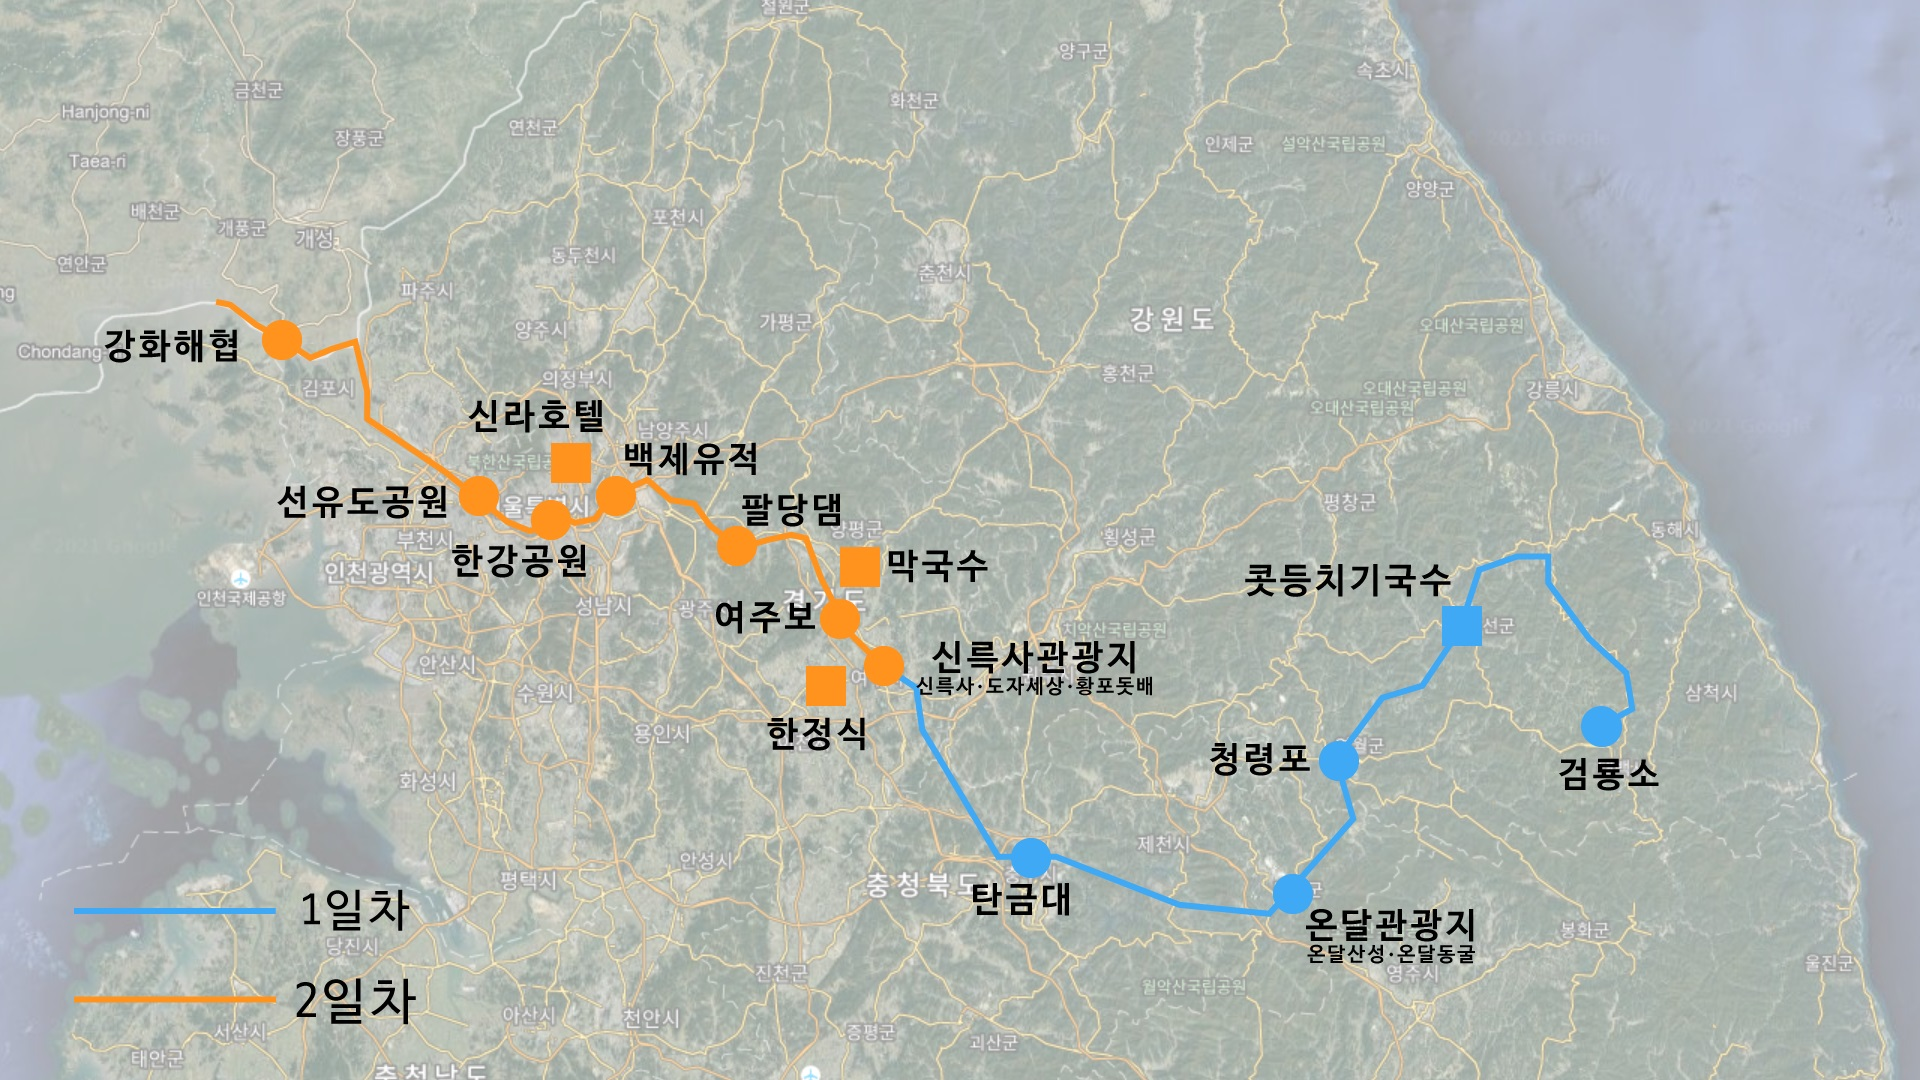
\includegraphics[width=1\textwidth]{img/전체-지도.jpg}
    \caption{지도에 나타낸 답사 경로\protect\footnotemark}
    \label{fig:path}
\end{figure}
\footnotetext{\href{https://www.google.com/maps/@37.4649392,127.9721805,279740m}{구글 지도 갈무리 후 편집}}

\subsection{1일차}
\begin{itemize}
    \item 직선 이동거리: 210km
    \item 경유 지역: 강원도 태백시, 정선군, 영월군, 충청북도 단양군, 충주시, 경기도 여주시
\end{itemize}


\begin{table}[ht]
    \begin{center}    
    \begin{tabular}{rl}
    \multicolumn{1}{l}{시간}     & \multicolumn{1}{l}{장소} \\ \hline
    \multicolumn{1}{r|}{05:00} & 태백 구문소 등산, 및 금대산   일출 \\
    \multicolumn{1}{r|}{11:00} & 정선 콧등치기   국수          \\
    \multicolumn{1}{r|}{12:00} & 영월 청령포 답사             \\
    \multicolumn{1}{r|}{15:00} & 단양   온달관광지 답사         \\
    \multicolumn{1}{r|}{17:00} & 충주   탄금대              \\
    \multicolumn{1}{r|}{19:00} & 여주   숙소              
    \end{tabular}
    \end{center}
\end{table}
\subsection{2일차}
\begin{itemize}
    \item 직선 이동거리: 150km (자전거 80km, 자동차 70km)
    \item 경유 지역: 경기도 여주시, 양평군, 남양주시, 서울특별시, 인천광역시 강화군
\end{itemize}

\begin{table}[ht]
    \begin{center}
    \begin{tabular}{rl}
    \multicolumn{1}{l}{시간}     & \multicolumn{1}{l}{장소} \\ \hline
    \multicolumn{1}{r|}{07:00} & 아침   여주 한정식         \\
    \multicolumn{1}{r|}{08:00} & 여주   도자세상과 신륵사      \\
    \multicolumn{1}{r|}{09:30} & 여주   황포돛배           \\
    \multicolumn{1}{r|}{10:00} & 여주보 이동, 자전거 대여.     \\
    \multicolumn{1}{r|}{10:30} & 점심   천서리막국수         \\
    \multicolumn{1}{r|}{14:00} & 양평 두물머리, 팔당댐 통과     \\
    \multicolumn{1}{r|}{15:00} & 서울 몽촌, 풍납토성         \\
    \multicolumn{1}{r|}{16:30} & 한강공원   통과           \\
    \multicolumn{1}{r|}{17:30} & 서울   선유도공원. 자전거 하차. \\
    \multicolumn{1}{r|}{18:30} & 저녁   신라호텔 팔선중식당. 일몰 \\
    \multicolumn{1}{r|}{20:30} & 강화   강화해협. 야경. 해산. 
    \end{tabular}   
    \end{center}
\end{table}
※빌린 자전거는 택배로 반납.



\chapter{1일차, 한강 상류}
\section{여행의 시작, 태백}
\subsection{이무기가 몸부림 친 곳, 검룡소}
서울을 가르는 거대한 물줄기, 한강은 어디서 시작되었을까? 
강원도 태백에는 1987년 국립지리원에서 인정받은 한강의 공식 발원지 검룡소가 있다. 
검룡소는 강원도 태백시 창죽동 금대봉 산기슭에 위치한다. 
이곳의 이름이 검룡소(儉龍沼)인 까닭은 이곳에 전해내려오는 전설과 관련이 깊다. 과거 서해에는 이무기가 살았다. 
이 이무기는 용이 되기 위해 한강의 강줄기를 거슬러 올라오기 시작했고, 결국 이곳 검룡소에 도착하게 된다. 
이무기가 용이 되기 위해 물이 솟는 굴에 들어가려 몸부림치는 바람에 검룡소 주변 물줄기의 모습이 마치 용틀임하는 것처럼 보이게 되었다고 한다. 

\subsection{한강의 발원지}
검룡소는 해발 800m에 위치해 있으며, 한강 하류까지 총 500km가 넘는 한강의 급수를 담당한다. 
검룡소에서는 사시사철 $9^\circ C$의 차가운 물이 흘러나오며, 
하루에 2,000톤 가량의 물이 굴에서 뿜어져 나와 계곡을 따라 흐른다. 
검룡소에서 시작한 물은 골지천으로 흐르는데, 이 골지천이 한강의 발원천이다. 

\begin{figure}[ht]
    \centering
    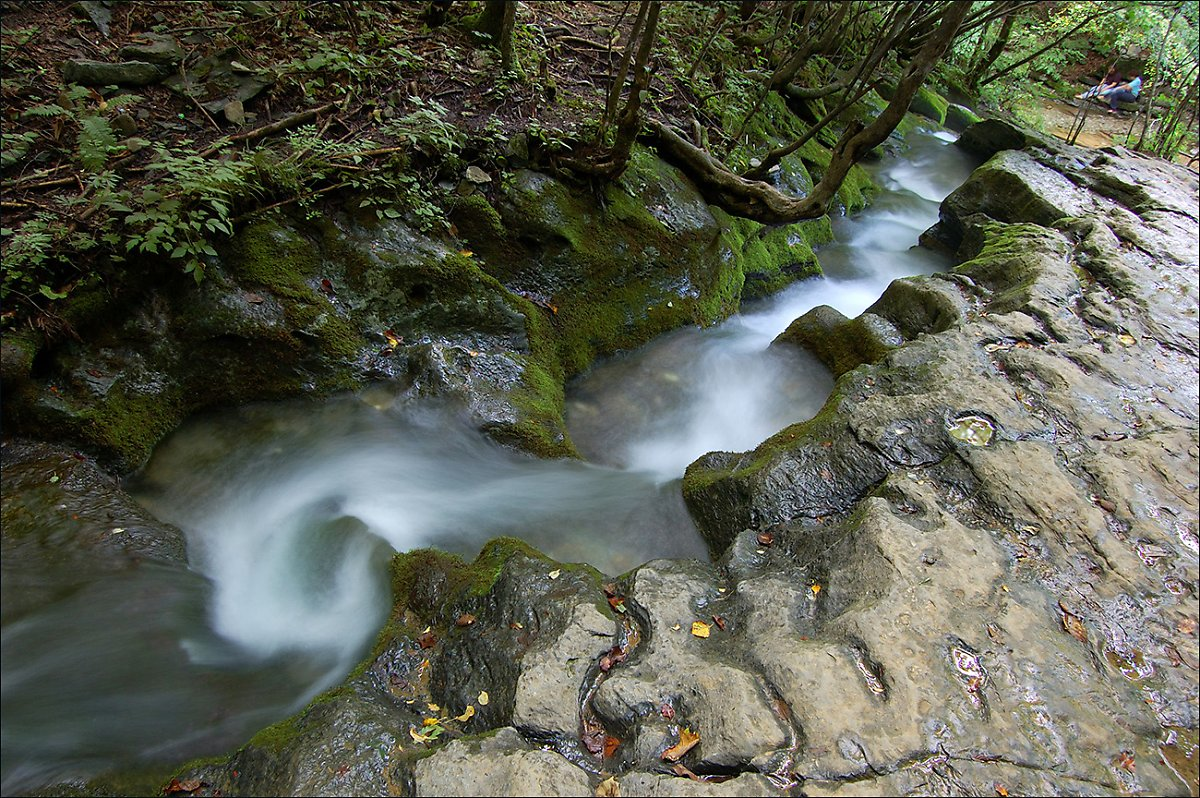
\includegraphics[width=.32\textwidth]{s_img/검룡소_사진.jpg}
    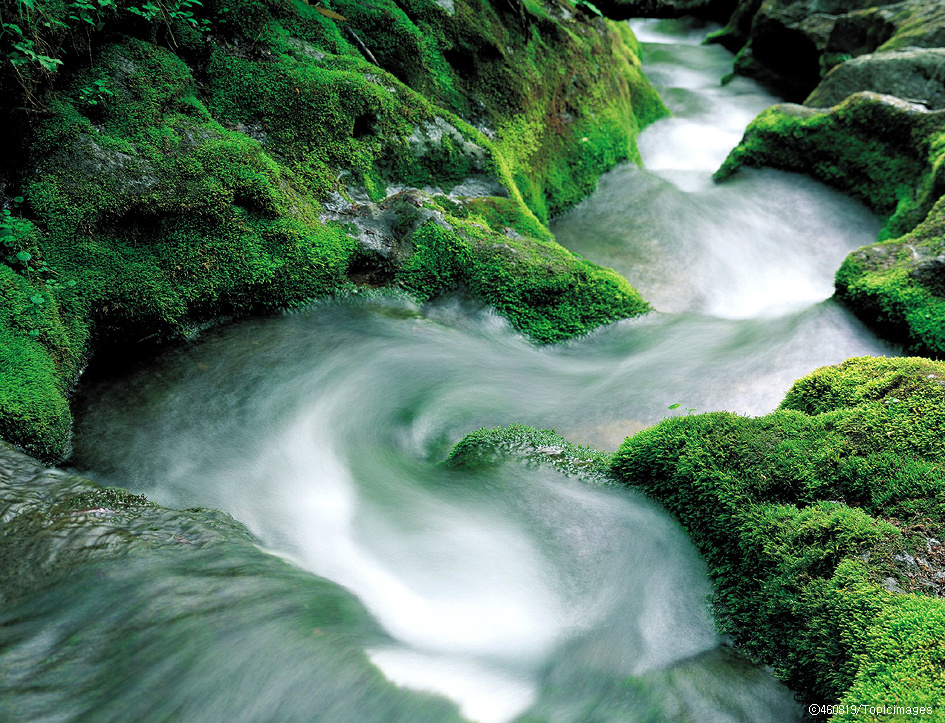
\includegraphics[width=.32\textwidth]{s_img/검룡소_사진2.jpeg}
    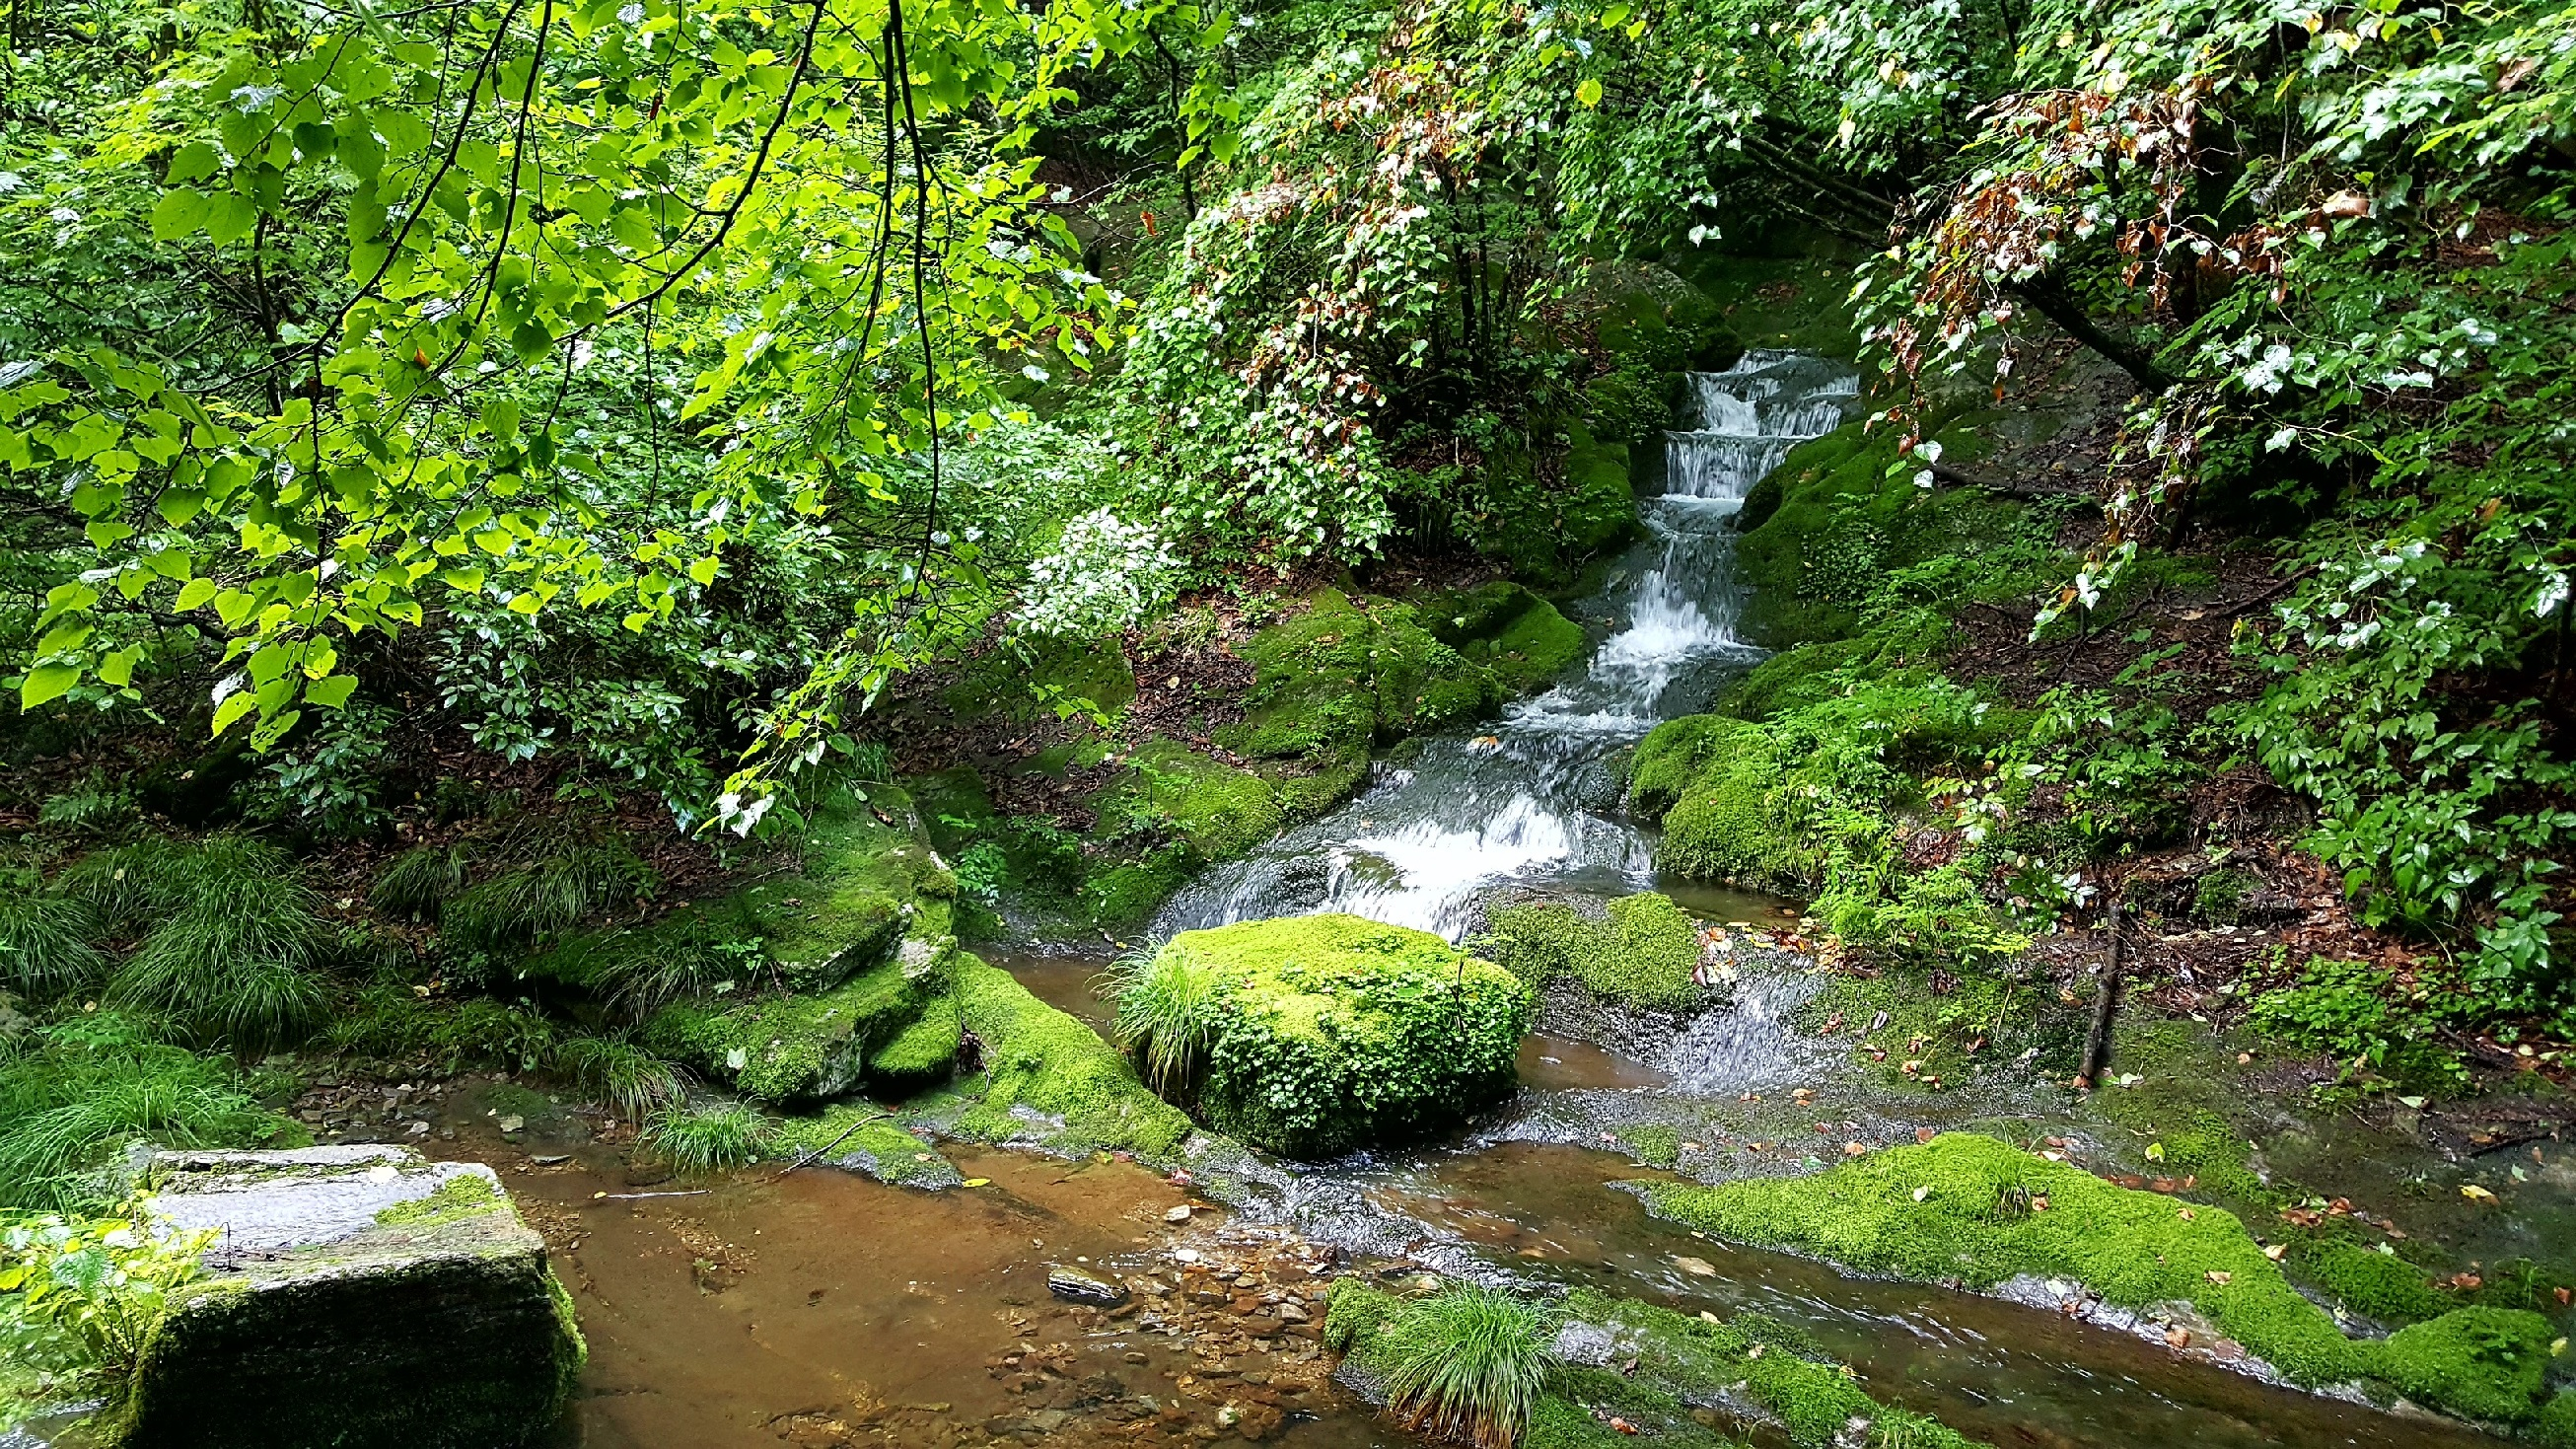
\includegraphics[width=.32\textwidth]{s_img/태백검룡소_사진_low.jpg}
    \caption{검룡소의 모습}
    \label{fig:my_label_s1}
 \end{figure}

\section{점심: 콧등치기국수 - 정선}
\subsection{메밀과 정선}
강원도 정선에서는 예로부터 메밀 농사를 많이 지었다. 
메밀은 척박한 땅에도 잘 자랐기 때문에 고추나 감자를 심고 남은 돌밭에 메밀을 심고는 했다. 
이마저도 메밀은 다른 작물과 심는 법이 달랐다. 
대개 작물을 심을 때 골을 켜고 씨앗을 심었다면, 메밀은 그저 밭에 씨앗을 뿌릴 뿐이었다. 
이곳 정선의 사람들은 그걸 `메밀을 푼다'고 했다. 메밀은 잘 자라는 것만큼이나 버릴 것 하나 없었다. 
메밀 잎은 나물로 무쳐 먹고, 줄기는 불쏘시개로 쓰기 알맞으며, 메밀 껍질 `달갱이'는 베개 속으로 사용했다.

정선의 먹을거리에는 메밀이 빠지지 않는다. 메밀국수를 비롯해 메밀묵, 메밀전병, 메밀전, 메밀국죽 등 
정선을 대표하는 메밀 먹거리들이다. 
이렇게 메밀로 만든 음식이 많음에도 메밀이 가진 고유의 맛과 모양 덕분에 매일 질리지 않고 메밀로 만든 음식을 즐길 수 있다. 

\begin{figure}[ht]
    \centering
    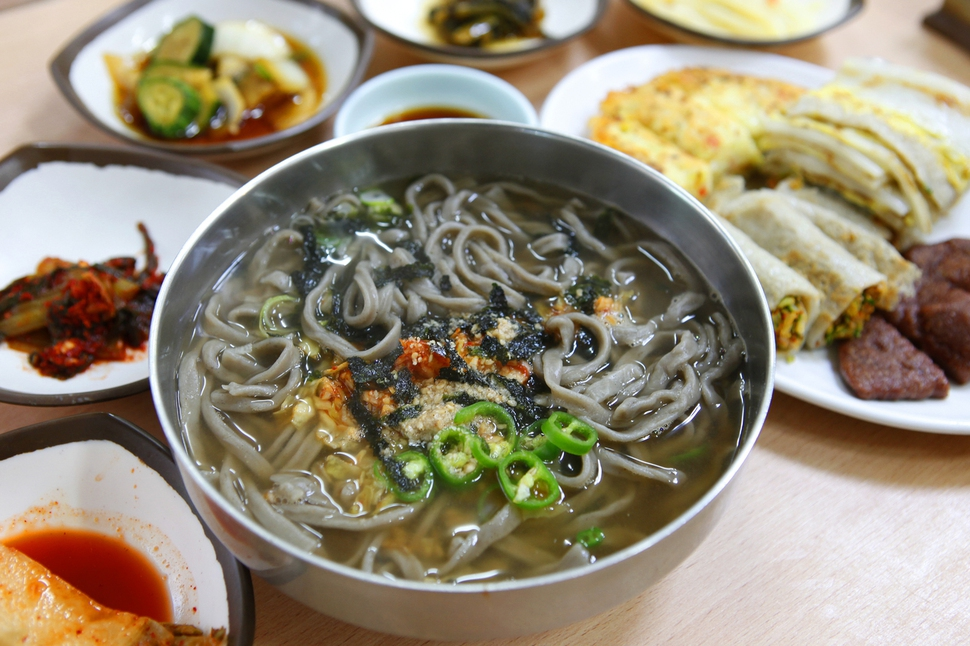
\includegraphics[width=.6\textwidth]{s_img/콧등치기국수_사진.JPG}
    \caption{콧등치기국수 사진}
    \label{fig:my_label_s2}
 \end{figure}

\subsection{메밀 국수와 콧등치기 국수}
메밀 국수를 시키면 메밀 반죽으로 만든 굵고 납작한 국수를 뜨근한 육수와 함께 준다. 
쫄깃한 면발은 고명으로 올라간 갓김치와 정말 잘 어울린다. 
그러나 정선에서 메밀 국수는 콧등치기 국수로 더 유명하다. 
정선아리랑연구소의 시인 진용선씨는 정선 문화의 대중화를 위해 메밀 국수에 콧등치기 국수라는 이름을 붙였다. 
잡지나 신문에 글을 쓸 때마다 콧등치기 국수란 말을 사용하여 요즈음에는 메밀 국수보다 콧등치기 국수란 말이 더 유명해졌다. 
메밀 국수의 다른 이름이 콧등치기 국수가 된 것은 퉁퉁한 면발이 자꾸 콧등을 친다며 붙어졌다. 


\section{조선의 불운한 왕 단종, 영월}
\subsection{삼면은 강으로 둘러쌓인 청령포}
청령포의 주변은 전형적인 감입곡류 하천의 형태를 띄고 있다. 
지반이 융기하면서 형성된 감입 곡류 하천은 측방 침식보다 하방 침식이 활발하게 나타나기 때문에 강의 폭보다는 수심이 깊은 형태를 띤다. 
또한 주변에서 하중도나 구하도, 우각호 등의 지형을 살펴볼 수 있다. 삼면이 강으로 둘러쌓여 있고, 
뒤는 암석 절벽으로 막혀 있어 청령포에 가는 방법은 오로지 배를 타고 강을 건너가는 것뿐이다. 
청령포를 둘러싼 서강이 과거 흐르던 방절리 주변 저지대에는 구하도와 곡류핵, 하안단구가 잘 보존되어 학술적으로 큰 의미가 있다.


\begin{figure}[ht]
    \centering
    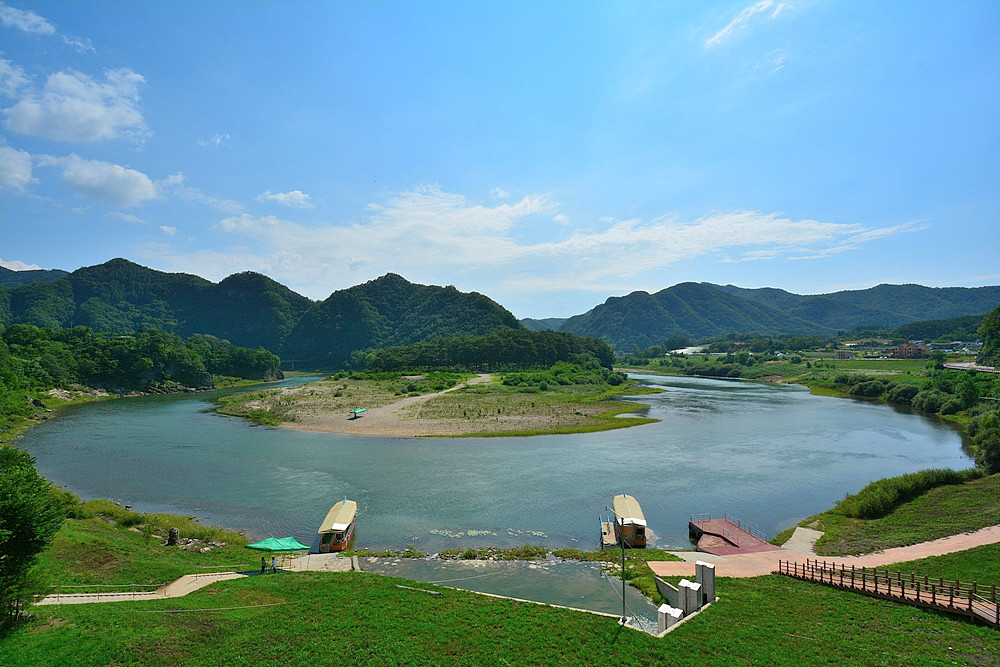
\includegraphics[width=.4\textwidth]{s_img/청령포_사진.jpeg}
    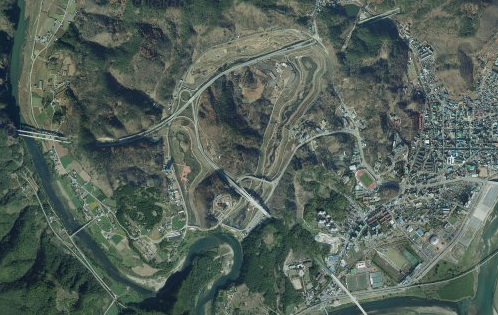
\includegraphics[width=.4\textwidth]{s_img/청령포_구하도.png}
    \caption{(좌)청령포 전경 $\quad$ (우)청령포 주위의 구하도\protect\footnotemark}
    \label{fig:my_label_s3}
 \end{figure}
 \footnotetext{\href{http://kko.to/zgW6gWkYM}{카카오맵 갈무리}}

 
\subsection{단종의 유배 생활}

앞서 설명한 바와 같이 이곳 청령포는 배를 타지 않고서는 나갈 수 없는 지형을 가지고 있다. 
이에 청령포는 1457년(세조 3년)에 단종이 세조에게 왕위를 빼앗기고 유배를 당했던 장소가 되었다. 
강나루 옆에는 단종의 유배길에 금부도사로 온 왕방연의 시비가 세워져 있다. 
당시 왕명을 수행할 수밖에 없었던 왕방연의 한없이 슬픈 마음이 비에 새겨져 있다. 
회단종이작시조(懷端宗而作時調) - ``천만리 머나먼 길에 고운님 여의옵고 내 마음 둘 데 없어 냇가에 앉았으니 저 물도 내 안과 같아서 울면서 밤길을 가더라.''
청령포 안에는 유배 당시 단종이 살았던 단종어가가 승정원일기의 기록을 토대로 복원되어 있다. 

이곳 단종어가 앞뜰에는 단종의 옛 집터를 기념하기 위해 영조 39년에 세운 비가 있다. 
비의 앞면에는 영조가 직접 하사한 ``단묘재본부시유지(端廟在本府時遺址)''라는 글이 써 있고, 
뒷면에는 ``歲皇明崇禎戊辰紀元後三癸未季秋泣涕敬書令原營竪石''라는 글이 써 있다. 
청룡포 서쪽 능선에는 망향탑이 있다. 이 망향탑은 열일곱 살 단종이 자신의 배우자 정순왕후 송 씨를 생각하며 주위에 돌을 쌓아 만든 탑이다. 
정순왕후 송 씨는 궁궐에서 쫓겨난 뒤 지금의 숭인동에 초가집을 짓고, 매일 아침저녁으로 동망봉에 올라 단종의 무사를 기원했으며, 
단종의 죽음을 알고는 매일 통곡하며 명복을 빌었다고 전해진다. 

\begin{figure}[ht]
    \centering
    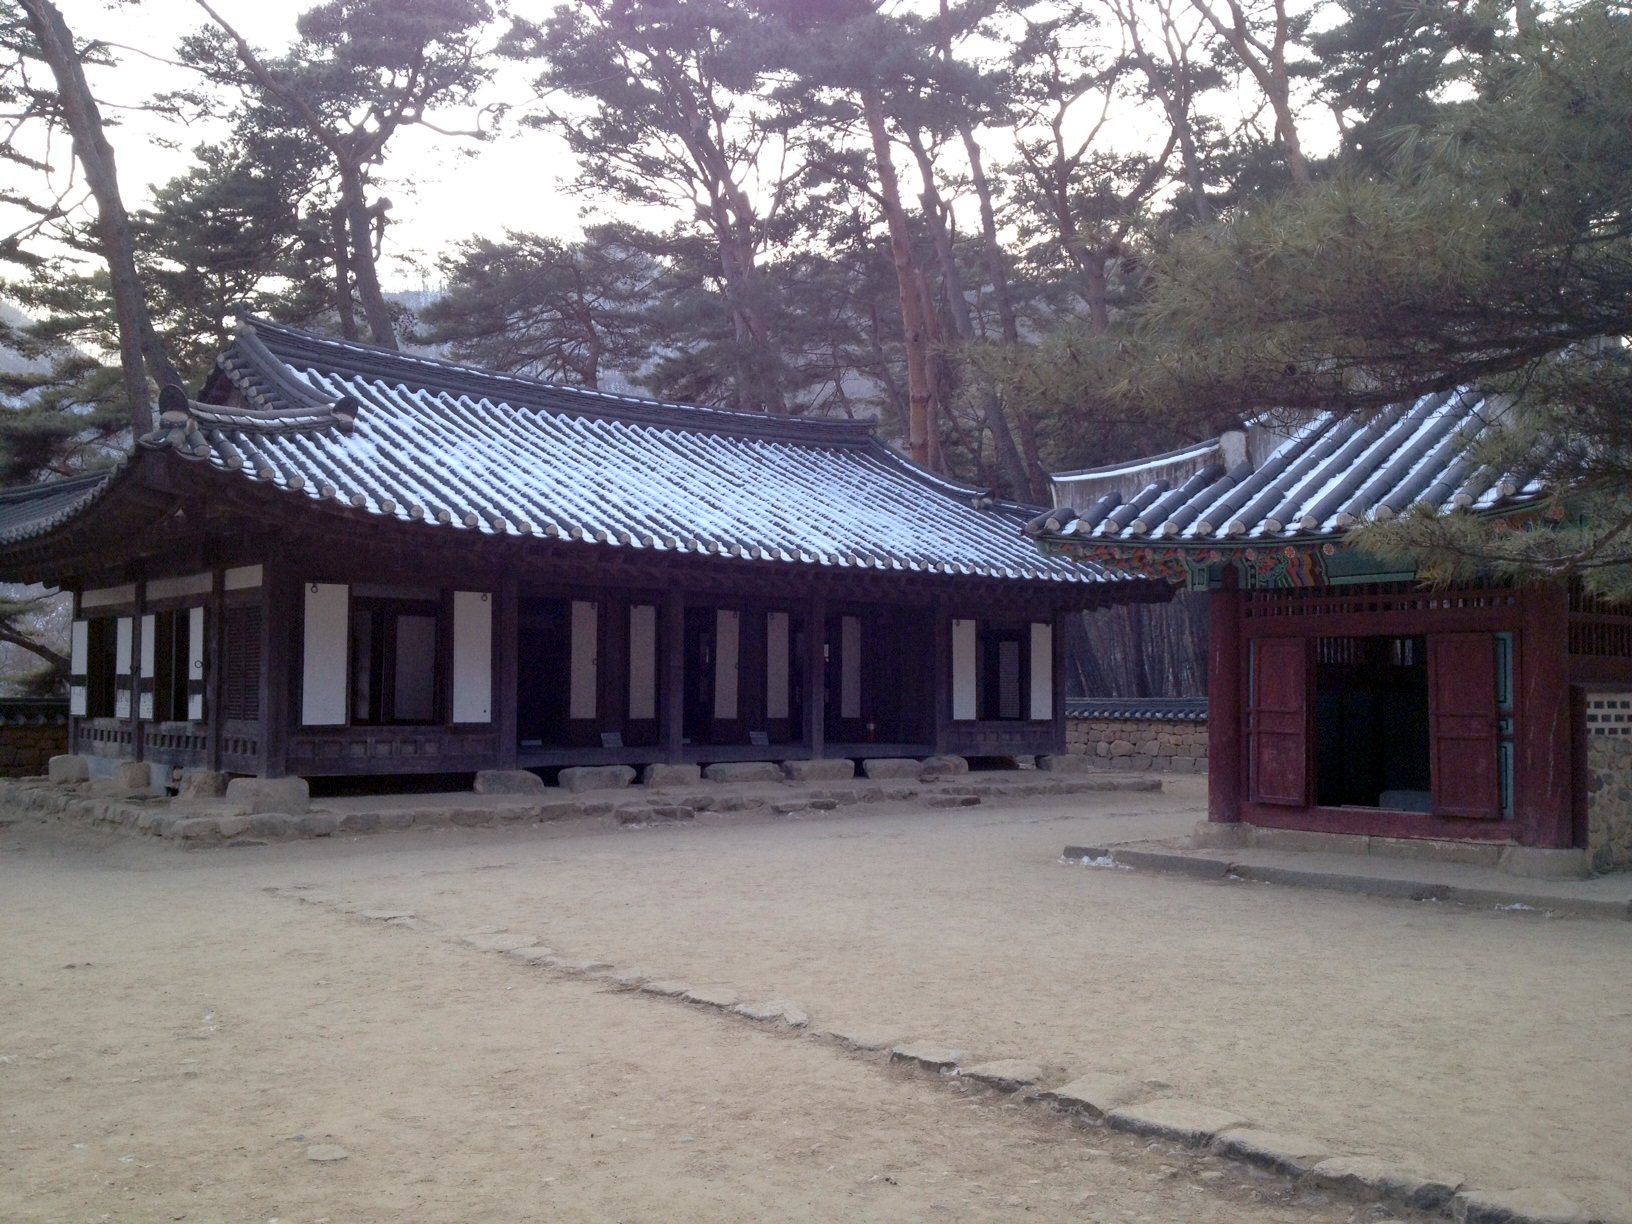
\includegraphics[width=.6\textwidth]{s_img/청령포_사진_2.JPG}
    \caption{청령포 내에 위치한 단종 어소. (단종이 유배되어 있던 곳) \protect\footnotemark}
    \label{fig:my_label_s31}
\end{figure}
\footnotetext{\href{https://commons.wikimedia.org/wiki/File:CheongRyeongpo_Eoso.JPG}{단종의 첫 유배지 청령포에 위치한 어소. $|$ 위키미디어 공용, 2012.01.11}}


\section{바보 온달과 평강 공주, 단양}
\subsection{평강 공주 전설}
고구려 평원왕의 딸이었던 평강 공주는 어려서부터 자주 울었고, 그때마다 아버지 평원왕은 바보 온달에게 시집보내겠다며 공주를 놀렸다. 
평강 공주가 16세가 되던 해에 평원왕이 공주를 상부(上部)의 고씨 가문에 시집보내려 하자, 
공주는 이를 거부하고 궁궐에서 뛰쳐나갔다. 공주는 어릴 적 귀가 빠지게 듣던 바보 온달을 찾아갔다. 
장님이었던 온달의 어머니는 찾아온 평강 공주의 향기와 부드러운 손을 만져보고는 이곳은 이렇게 귀하신 분이 오실 곳이 아니라 하였다. 
때마침 집에 온 온달마저도 어린 여자가 할 행동이 아니라며 공주를 강하게 거부했다. 
그러나 공주는 포기하지 않고 다음날 아침에 온달 모자를 다시 설득했고, 마침내 그 둘은 혼인하였다. 
평강 공주는 가져온 팔찌를 팔아 살림을 장만하고 말을 정성스레 키웠다. 그리고 그 말은 온달과 함께 전투에서 큰 공을 세웠다. 
590년, 온달은 아단성에서 신라와 싸우다 전사해 관에 들어가게 되었는데, 
그 관은 아무리 옮기려 해도 꿈적도 하지 않았다. 
이에 평강이 관을 어루만지며 이미 생사는 정해졌으니 이만 돌아가자고 하자, 그제서야 관이 움직이기 시작했다. 


\begin{figure}[ht]
    \centering
    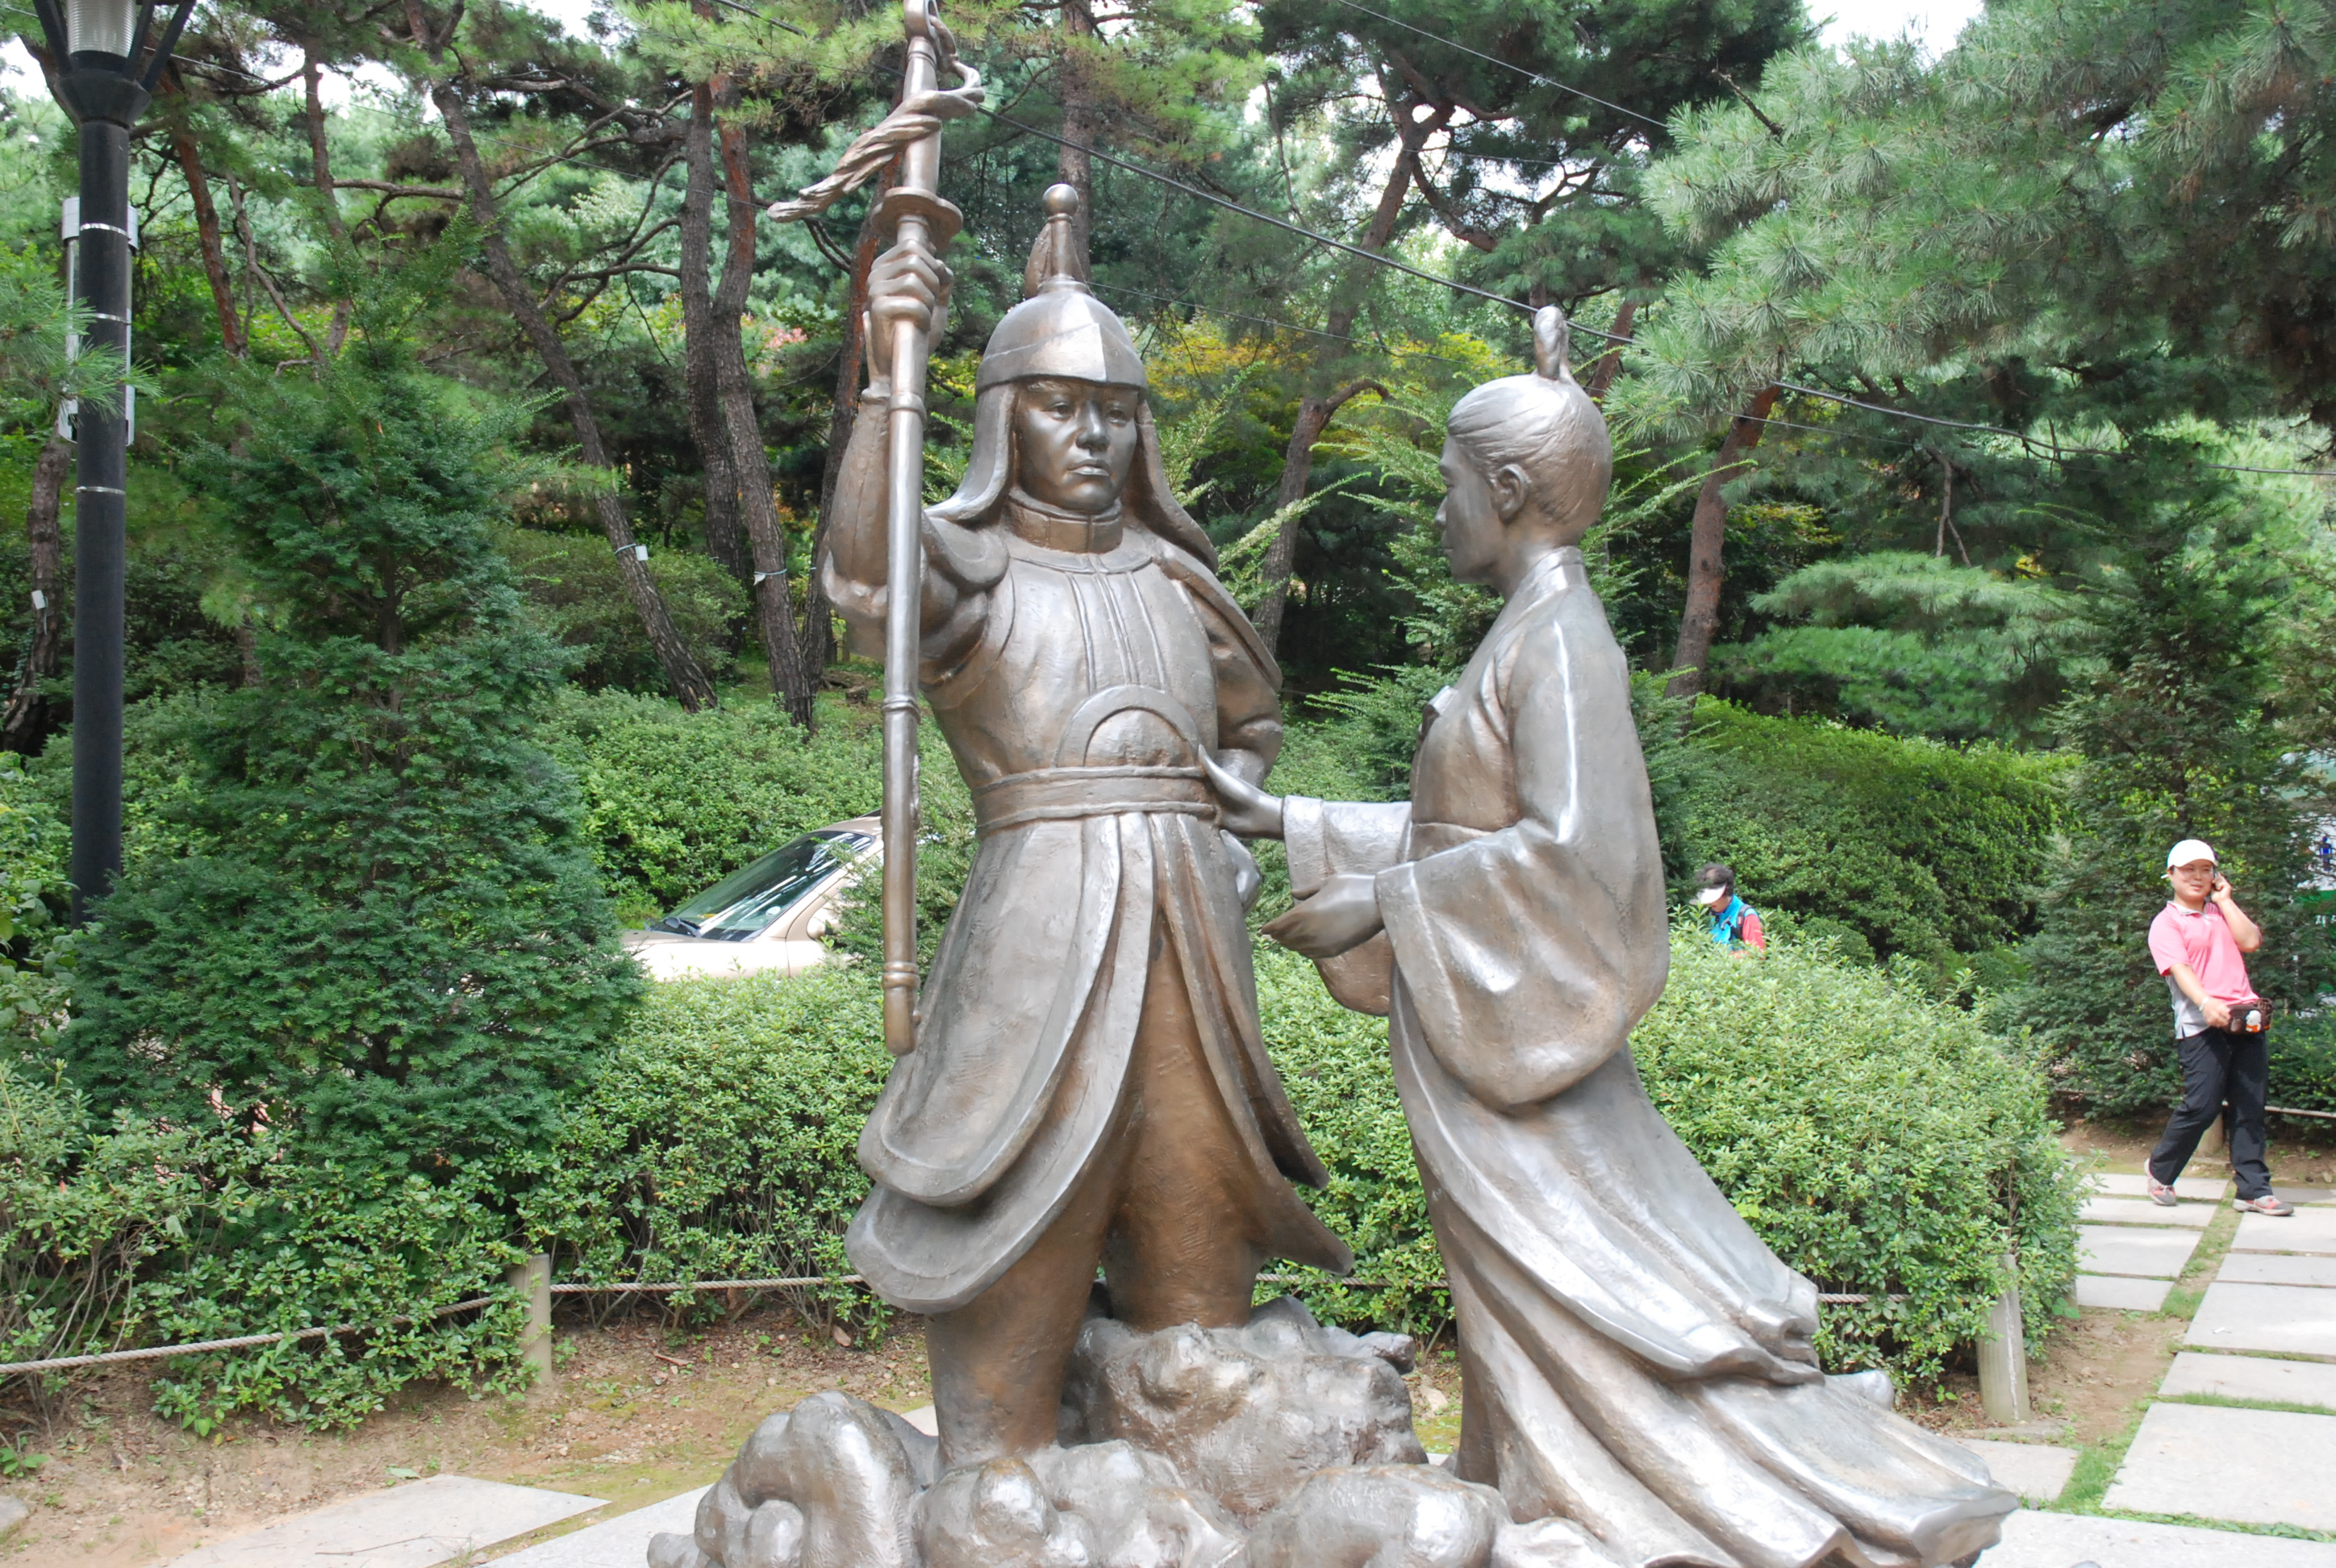
\includegraphics[width=.6\textwidth]{s_img/온달_사진.jpg}
    \caption{온달 동상의 모습}
    \label{fig:my_label_s4}
 \end{figure}

\subsection{온달 공원 탐방}
$<$연개소문$>$, $<$태왕사신기$>$, $<$바람의 나라$>$, $<$천추태후$>$ 등의 드라마가 제작된 이곳 온달 공원은 
온달 전시관을 비롯해 온달 산성, 온달 동굴 등 명승이 모여있는 곳이다. 
온달 공원 이곳 저곳에는 실제 촬영을 위해 사용된 세트장이 아직 남아있는데, 촬영에 사용된 의상이나 소품도 함께 배치되어 있어 
드라마 촬영 현장을 생동감 넘치게 즐길 수 있다. 
온달 전시관 옆에는 석회질 동굴인 온달 동굴이 있다. 
온달 동굴은 1979년 6월에 천연기념물 261호로 지정된 총길이 700m 가량의 석회동굴이다. 
이름이 온달 동굴인 까닭은 온달 장군이 쌓은 온달 산성 아래 위치해 있기 때문이다. 
이 동굴의 입구는 남한강변에 위치해 강수 등의 이유로 수위가 높아지면 동굴이 물에 잠기는 까닭에 내부에 사는 생물은 찾아볼 수 없다. 
동굴 내부는 꾸준히 물이 흐르기 때문에 단조로운 형태를 띄며 식생도 다양하지 않다. 
그러나 동굴 내부에서 석순을 어렵지 않게 찾아볼 수 있다. 


온달 산성의 다른 이름은 아단성으로 실제 온달이 신라와 싸우다 전사한 장소이다. 
성산의 정산 부근을 돌로 쌓아 만든 둘레 683m 정도의 소규모 산성으로, 
내외부에서 삼국시대 유물과 우물터, 배수구 등이 발견된다. 
한강은, 한반도의 중부를 흐르는 강으로 삼국시대 삼국의 접경지대였다. 
또한, 강 주변의 비옥한 평야지대, 수운을 이용할 수 있어 교통이 유리하고, 중국과 교역할 수 있다는 점에서 삼국이 모두 탐내는 곳이었다.
끝내 한강을 차지한 신라가 삼국을 통일했다는 점에서, 비록 결과론적이지만
한강의 지배자가 한반도의 지배자가 된 것이다.
남한강이 내려다 보이는 산자락에 위치한 온달산성은, 
이러한 삼국의 각축전을 잘 보여주는 장소이다.
\footnote{\href{https://www.edunet.net/nedu/contsvc/viewWkstCont.do?clss_id=CLSS0000000362&menu_id=81&contents_id=1d7c0c64-bc0f-45e7-8f4d-82a7bb00cc97&svc_clss_id=CLSS0000072410&contents_openapi=naverdic}
{에듀넷 T 클리어 $>$ 교과주제 학습자료 $>$ 사회 $>$ 삼국 시대와 동아시아의 재편 $>$ 삼국시대 한강 유역의 의미 $|$ 한국교육학술정보원}}


\begin{figure}[ht]
    \centering
    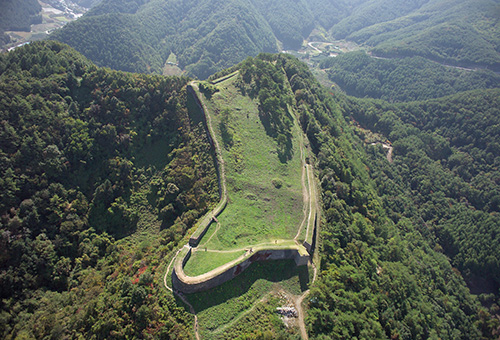
\includegraphics[width=.4\textwidth]{s_img/온달산성_사진.JPG}
    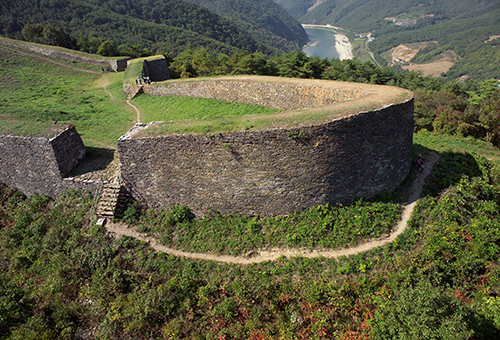
\includegraphics[width=.4\textwidth]{s_img/온달산성_사진2.JPG}
    \caption{하늘에서 본 온달산성 전경}
    \label{fig:my_label_s5}
 \end{figure}

\section{쓰라린 패배의 기억, 충주}
\subsection{충주 탄금대와 임진왜란}
충주 탄금대는 임진왜란에서 탄금대 전투가 일어난 지역으로 유명하다. 임진왜란 당시 부산진성과 동래성이 함락되고 파죽지세로 상주마저 함락되었다. 이에 선조는 신립에게 왜군 방어 임무를 내렸고, 신립은 그렇게 문경으로 출동했다. 신립과 함께한 김여물은 문경새재의 언덕과 바위를 방패 삼아 궁병으로 공격하자고 했으나, 신립은 충주의 달천 평야에서 궁기병을 활용해 공격하자고 했다. 이는 신립이 일본군의 대부분이 보병이므로, 조선의 기병이 일본을 상대로 우위를 점할 수 있을 것이라 생각했기 때문이었다. 그러나 이는 틀린 추측이었다. 달천 평야의 논밭은 젖어있어서 기병이 활동하기 어려운 지형이었고, 결국 일본군에게 참패하고 만다. 그 결과 신립은 탄금대에 몸을 던져 익사했다고 전해진다. 

\chapter{2일차, 한강 중류 (경기 동부)}
\section{아침: 한정식 - 여주·이천 평야}
충주를 거쳐 원주를 통과한 남한강은 여주, 이천 일대의 넓은 평야지대를 마주한다. 
감입곡류하천의 흔적은 온데 간데 없고, ‘백석리도’, ‘양도’ 등 큰 하중도가 눈에 들어온다.
일부 사행하천의 모습도 보인다.

\begin{figure}
    \centering
    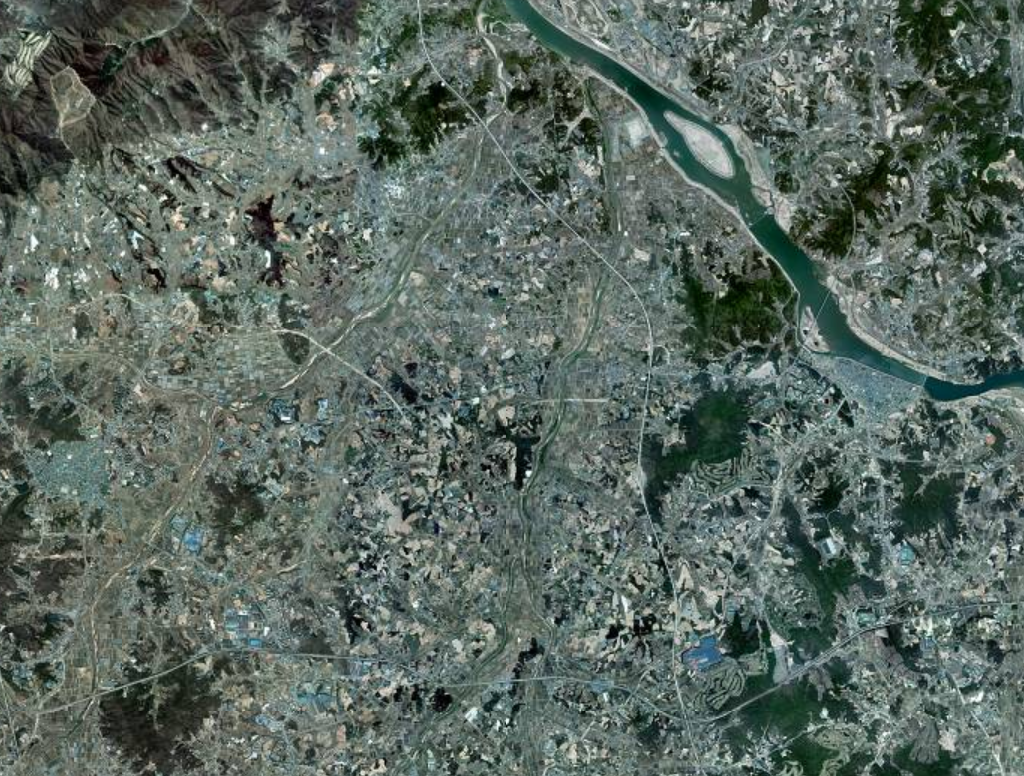
\includegraphics[width=.6\textwidth]{img/여주이천평야.PNG}
    \caption{여주·이천 평야의 위성사진\protect\footnotemark}
    \label{fig:my_label}
\end{figure}

\footnotetext{\href{http://kko.to/-Cb9A-mDT}{카카오맵 갈무리}}

이 여주, 이천 일대는 
광주산맥, 태백산맥, 차령산맥으로 둘러싸인 분지로써,
그 사이로 남한강이 동남쪽에서 북서쪽으로 흐르고 있다.
남한강의 퇴적 작용의 의해 형성된 충적평야가 여주시, 이천시 경계에 북하천, 양화천을 따라 넓게 펼처져 왔다.
이 평야에서는 예로부터 논농사를 지어 왔다.
\footnote{대표적인 증거로, 남한강변 구릉에 위치한 \href{https://terms.naver.com/entry.naver?docId=1793906&cid=49217&categoryId=49217}{혼암리 선사 유적지}에서 탄화된 벼가 발견되었다.}


또한, 이 쌀은 남한강 수운을 통해 쉽게 한양까지 운반되었고, 특히 임금님께 진상될 정도로 높은 품질을 자랑했다고 한다.
특히 이 평야에서 생산되는 쌀은, 지리 교과서에서 우리나라의 대표적인 지리적 표시제 예시로 소개될 만큼 전국적으로 명성이 높다.
따라서 이러한 의미로 아침식사는 여주 한정식으로 결정하였다.
 
% caption 안에 footnote 안들어가짐 우회법
%https://stackoverflow.com/questions/2888817/footnotes-for-tables-in-latex
%https://ko.overleaf.com/learn/latex/Footnotes

\begin{figure}
    \centering
    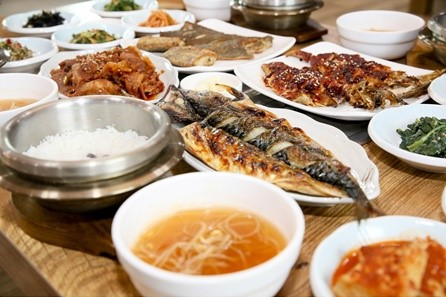
\includegraphics[width=.6\textwidth]{img/한정식.jpg}
    \caption{아침: 한정식 \protect\footnotemark}
    \label{fig:my_labe2}
\end{figure}
\footnotetext{\href{http://www.kbanker.co.kr/news/articleView.html?idxno=83122}{경기도 여주, 아름다운 관광명소에 쌀밥집 식도락까지, 여주 아울렛 맛집 ‘수라온한정식’ $|$ 대한금융신문 2019.05.28}}
뜬금없이 한반도 내륙에, 평야가 발달한 이유가 무엇일까?
특히. 이 일대의 산지를 이루고 있는 화강암은 풍화에 약한 장석과 운모로 되어 있어, 
쉽게 차별침식 받아 이러한 층적 평야를 만드는 데에 일조한 것이다.
이와 비슷한 곳으로 논산평야, 미호평야 등이 있다.


\footnote{ \href{https://www.yeoju.go.kr/history/main.jsp}{여주시사 $>$ 자연과 인문환경 $>$ 자연환경 $>$ 여주시의 지형 $|$ 여주시, 2015}}

\section{여주 도자마당 - 여주, 이천, 광주의 도자기}
여주, 이천, 광주 지역은 도자기로 유명하다. 이들 지역에서는 매년 도자기 축제가 열리며, 도자 비엔날레는 3개 시가 번갈아 가면서 개최한다.
우리가 갈 곳은 신륵사 옆에 위치한 여주 도자세상이다.
 이곳에는 도자기 판매처, 그리고 도자 작품을 전시하고 있는 반달 미술관이 있으며, 앞 뜰에서는 매년 도자기 축제가 열린다. 
 각종 전시 관람, 도자기 구입과 제작 체험 등을 할 수 있다.

 \footnotetext{\href{https://www.kocef.org/02museum/2021_04.asp}{한국도자제단 $>$ 강신봉 제6달항아리전 갈무리}}
 \begin{figure}
    \centering
    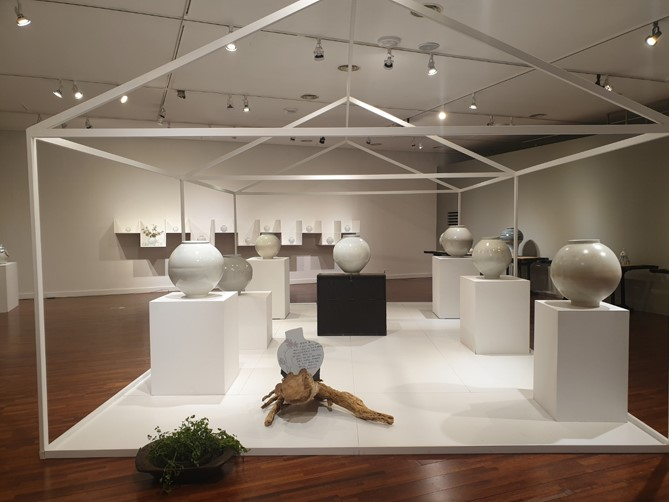
\includegraphics[width=.4\textwidth]{img/도자전.jpg}
    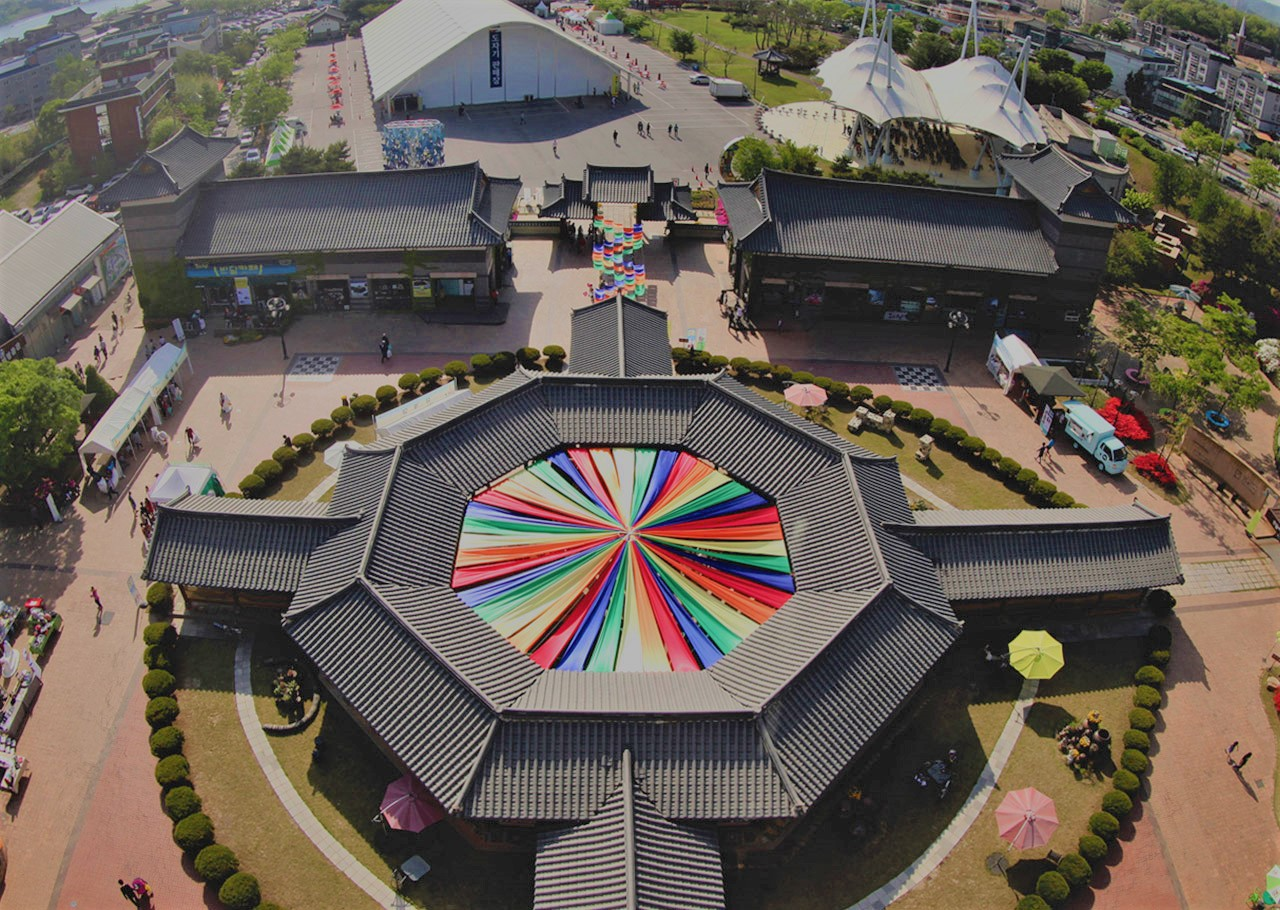
\includegraphics[width=.4\textwidth]{img/여주도자세상.jpg}
    \caption{(좌)도자세상 내 반달미술관\protect\footnotemark $\quad$ (우)어주도자세상 전경\protect\footnotemark}
    \label{fig:my_labe3}
\end{figure}
\footnotetext{\href{http://www.yjceramic.or.kr/2020/main/main.html}{제 32회 여주도자기축제 누리집 갈무리}}

또한, 장석, 운모류의 조암광물들은 화학적 풍화작용을 받아 점토를 형성하는데,
이는  여주, 이천, 광주 일대를 도자기 산업을 발달시키는 근간이 되었다.

특히, 일대의 지형이 완만한 경사가 져 있고
북쪽에 산이 있어 북서풍을 차단해 따뜻해 전통가마가 들어오기 좋은 조건을 갖고 있으며,
가마의 원료인 점토, 백자의 원료인 양질의 백토를 쉽게 구할 수 있었다.
또한 남한강 수운을 통해 영월, 충주, 청풍 지역의 도자기 원료를 쉽게 구할 수 있었다.

이곳에서 생산된 도자기는 남한강을 통해 한양으로 운반되었으며,
특히 상대적으로 하류 지역인 광주에는 왕실 전용 도자기 공장인 광주 관요가 있었다.
일제강점기를 거치며 일본 공장제 자기의 유입, 문화말살정책 등으로 쇠퇴를 겪었으나,
광복 후 60~70년대, 일본, 유럽 수출로 인해 빠르게 회복된다.
일본에 의해 부침을 겪은 도자기 산업이 일본에 의해 부흥했다는 점은, 우리 역사의 안타까운 점인 것 같다.
\footnote{\href{https://memory.library.kr/items/show/37951}{이천도자 利川陶磁 22-23p, 44-45p $|$ 이천시, 2006.02.01}}
\footnote{ \href{https://www.yeoju.go.kr/history/main.jsp}{여주시사 $>$ 총론 $>$ 위치와 연혁 $>$ 전국 생활도자기 산업의 메카 $|$ 여주시, 2015}}

\subsection{정보}

\begin{itemize}
\item 입장료: 무료
\item 반달미술관 관람시간: 09:00 $\sim$ 18:00 (매주 월요일 휴관)
\item 위치: 경기 여주시 천송동 297-1
\end{itemize}

\section{신륵사}
그 다음으로 둘러볼 곳은, 도자마당 바로 옆에 있는신륵사이다. 신륵사는 남한강변에 바로 붙어 있는 사찰이다. 
신륵이라는 이름 안에는, 날뛰는 용마(龍馬)를 나웅선사(혹은 인당대사)가 막았다는 전설이 있다.
강 건너편 바위 이름인 마암(馬巖)에서도 이 전설을 읽을 수 있다.


한편 신륵사 다층전탑 일대에 서면 남한강의 풍광이 한눈에 들어와 방문객들의 눈길을 끈다. 
특히, 이 탑은 보물 제 226호로써, 현존 유일의 고려시대 전탑이다.\footnote{
\href{https://terms.naver.com/entry.naver?docId=560144&cid=46656&categoryId=46656}{여주 신륵사 다층전탑 $|$ 한국민족문화대백과, 한국학중앙연구원}} 
 
 \footnotetext{\href{http://weekly.cnbnews.com/news/article.html?no=137111}{[겸재 그림 길 (66) 황려호] 여주 신륵사의 흑마(驪)와 재갈(勒)에 얽힌 사연들 $|$ 문화경제, 2020.11.27}}
 \begin{figure}
    \centering
    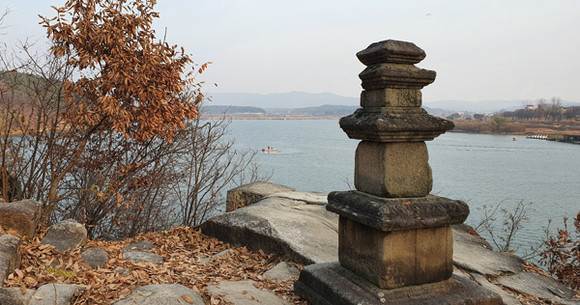
\includegraphics[width=.4\textwidth]{img/신륵사 삼층석탑.jpg}
    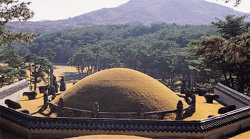
\includegraphics[width=.4\textwidth]{img/영릉.jpg}
    \caption{(좌)신륵사 삼층석탑에서 바라본 남한강\protect\footnotemark  $\quad$ (우)세종과 비 소헌왕후의 합장릉인 영릉(英陵)\protect\footnotemark}
    \label{fig:my_labe5}
\end{figure}
\footnotetext{\label{yeongreung}\href{https://weekly.donga.com/List/Series/3/99/11/76610/1}{한양 100리 밖 뱃길로 하루 행차 길 $|$ 주간동아 2005.06.17}}

특히, 조선 예종 시기, 세종대왕릉이 서울 대모산 옆(현 국정원 근처)에서 여주로 이전해 올 때,
이 왕릉을 수호하는 원찰로 이 사찰로 지정되면서 더 유명해졌다.
조선의 법전인 경국대전이 따르면 본래 왕릉은 한양에서 100리 이내에 지어야 했다. 
\footnote{\ref{yeongreung}}
이는 왕의 1일 행차 가능 거리가 100리이기 때문이다.
하지만 여주는 서울에서 100리보다 멀리 떨어져 있음에도, 남한강 수운을 이용할 수 있으므로,
위 규칙의 예외가 된 것이다.

\subsection{정보}
\begin{itemize}
    \item 입장료: 대인 3000원, 청소년 맟 군경 2200원, 어린이 1500원 
    \footnote{\href{http://www.silleuksa.org/}{신륵사 누리집}}
    \item 연중 무휴
    \item 위치: 경기 여주시 신륵사길 73-1
\end{itemize}

\section{황포돛배 - 한강의 수운}

우리나라는, 중국과 대조적이게도 육상교통이 발달하지 못했다. 이는 세 가지 이유로 압축된다.
첫째, 산이 많아 도로 건설에 어려움이 많았다. 
둘째, 침략에 취약하다는, 도로의 역기능 때문에 도로 건설을 꺼렸다. (무도즉안전, 無道則安全)
셋째, 농업 위주 경제$+$적은 생산량과 작은 국토로써 상공업의 발달이 지연되면서 도로 교통의 필요성이 적었다.
그에 비해, 큰 강과 바다를 이용한 수운이 매우 발달했다. 조선에서는 조세를 배를 통해 운반했다. 
\footnote{\href{http://encykorea.aks.ac.kr/Contents/Item/E0006539}{국토개발(國土開發) $|$ 한국민족문화대백과사전, 한국학연구원}}


따라서, 조선의 강은 오늘날의 경부고속도로의 역할을 한 것이다. 강을 따라 물자가 오갔고, 사람이 움직였다.
특히 한강은, 수도 한양을 흐르는 강으로써 그 중요도가 컸다. 특히 남한강은 영남지방과 연계되었다. 
조선시대 당시 여주에서 한양까지는 2일(순방향), 5일(역방향)이 걸렸다고 한다.
한강변을 따라 세금 창고, 나루터들이 들어섰고, 현재는 그 터만 남아 있다.


한강을 통한 수운은, 일제강점기 도로가 들어서며 쇠퇴하였고, 
여주$\cdot$이천 지역에서는 지금은 없어진 수려선 철도가 기폭제 역할을 했다.
\footnote{ \href{https://www.yeoju.go.kr/history/jsp/Theme/Theme.jsp?BC_ID=a0085}{여주시사 $>$ 자연과 인문환경 $>$ 인문환경 $>$ 교통과 통신 $>$ 내륙수로 교통과 나루터 $|$ 여주시, 2015}}

\begin{figure}
    \centering
    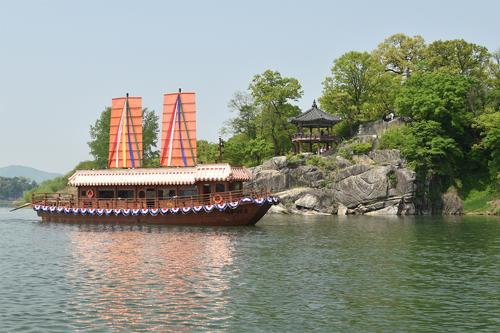
\includegraphics[width=.6\textwidth]{img/황포돛배.jpg}
    \caption{신륵사 앞을 가로지르는 황포돛배\protect\footnotemark}
    \label{fig:my_labe6}
\end{figure}
\footnotetext{\label{whangpo}\href{https://www.yeoju.go.kr/culture/content/view/2/menu/1757?contentIdx=132}{여주시 문화관광 $>$ 테마여행 $>$ 황포돛배}}


조선시대 대표 운송수단인 황포돛배를, 신륵사 건너편 금모래은모래 유원지에서 탑승할 수 있다. 
안타깝게도, 현재 운행하고 있는 배는 겉만 돛배이고 사실 기름으로 움직이는 배이다.
돛배에 올라 남한강 물살을 가로지르며, 기분만이라도 내 보자.
과거 조상들의 삶이 담긴 남한강을 달리며 그들을 되돌아 보자.

\subsection{정보}
\begin{itemize}
    \item 요금: 대인 6000원, 소인 4000원 \footnote{\ref{whangpo}}
    \item (매주 월요일 운휴)
    \item 위치: 경기 여주시 연양동 444
\end{itemize}

\section{한강 자전거길과 여주·이포보 - 4대강 사업}

한강 하면 빼 놓을 수 없는 것이 바로 4대강 사업이다.
이명박 정부는 국책사업으로 4대강 정비 사업을 벌였다.
수해 예방, 수자원 학보, 수질 개선, 지역 발전 등을 목표로 한 이 사업은,
남한강의 모습을 $180^\circ$ 전환했다.
얕은 여울, 넓은 강변 모래밭은 사라졌고, 그 자리에는 몇 $m$ 깊이로 파인 강바닥과, 수변공원, 그리고 보가 들어섰다.
이 일대 마을의 논을 빌려 남한강 준설토가 쌓였고,
아직도 다 팔리지 않아 주변 자치단체의 속을 썩이고 있다.
\footnote{\href{https://news.jtbc.joins.com/article/article.aspx?news_id=NB10593178}{[탐사플러스] 다시 쌓이는 4대강 준설토…예산 2천억 날려 $|$ JTBC, 2014.09.30}}
또한, 서식지가 파괴된 동야하루살이 때가 시내로 돌격하는 안타까운 일들이 벌어지기도 했다.
\footnote{\href{http://news.khan.co.kr/kh_news/khan_art_view.html?artid=201803201448001&code=620109}{봄철 불청객 '동양하루살이' 또 출현 $|$ 경향신문, 2018.03.20}}

한편, 사업으로 조성된 수변 공원은, 이 일대 시민들의 휴식처 역할을 독특히 하고 있다.
또한, 수변공원이 조성되면서 같이 조성된 국토 종주 자전거길로 인하여 수많은 사람들이 남한강으로 몰려 들었고,
강변에는 이들을 겨냥한 편의점이나 게스트 하우스 등 관련 산업들이 활성화되는 분위기다.
남한강변의 유명한 막국수 집에는, 이명박 젼 대통령의 친필 싸인이 자랑스럽게 걸려 있어,
이 사업이 지역에 야기한 파급 효과를 지례 짐작해 볼 수 있었다.
\footnote{\href{https://blog.naver.com/lovelyiii/221577715597}{여주 흥원막국수 | 네이버 블로그 행복한 여우, 2019.07.04 외 다수}}

\begin{figure}
    \centering
    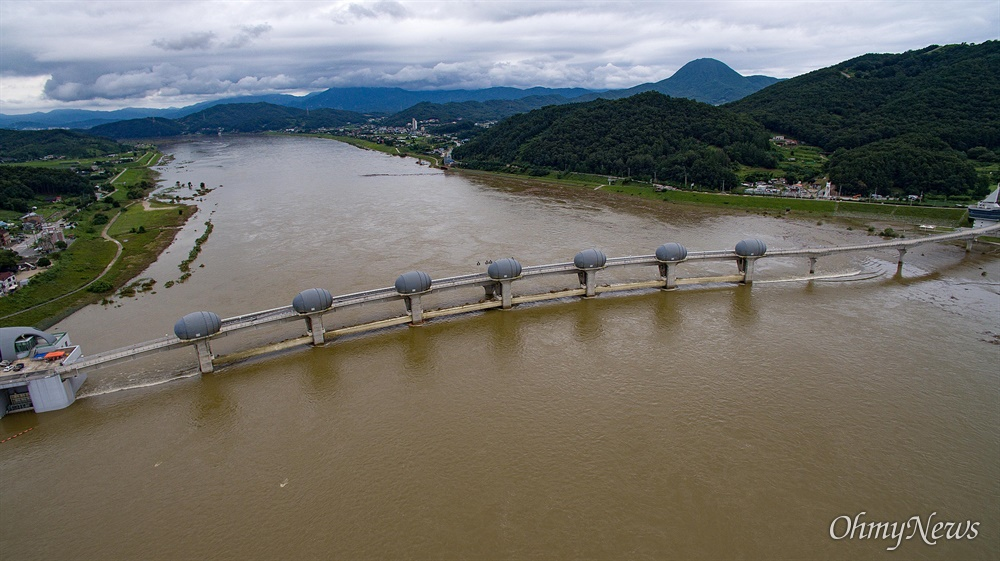
\includegraphics[width=.6\textwidth]{img/여주보.jpg}
    \caption{여주보의 모습. 국토종주 자전거길은 여주보 위를 통과한다. \protect\footnotemark}
    \label{fig:my_labe7}
\end{figure}
\footnotetext{\href{http://www.ohmynews.com/NWS_Web/OhmyPhoto/2020/at_pg.aspx?CNTN_CD=A0002665590}{[오마이포토] 수문 열고 황토물 흘려보내는 여주보와 이포보 $|$ 오마이뉴스, 2020.08.10}}


우리는 이제부터 자전거를 타고, 4대강 자전거길을 따라 하류로 향할 것이다.
여주부터 서울까지는 자전거 도로가 매우 잘 닦여 있는 편이다.
게다가, 양평부터는 구 중앙선 철도를 활용하기 때문에, 더더욱 선형이 좋다.
여주보에서 팔당댐까지는 자전거길로 $50km$ 정도 떨어져 있다. 
포털 사이트 지도에서는 3시간 59분이 소요될 것으로 예상하고 있다.
차로는 1시간이 걸리는 거리다.

\subsection{정보}
\begin{itemize}
    \item 요금: 무료
    \item 연중무휴
    \item 위치(여주보): 경기 여주시 능서면 왕대리 1008 
\end{itemize}

\section{점심: 천서리막국수}


\begin{figure}
    \centering
    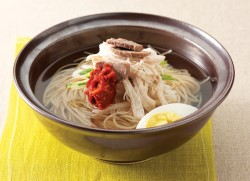
\includegraphics[width=.6\textwidth]{img/막국수.jpg}
    \caption{천서리막국수\protect\footnotemark}
    \label{fig:my_labe71}
\end{figure}
\footnotetext{\href{https://terms.naver.com/entry.naver?docId=1627391&cid=48179&categoryId=48238}{[천서리막국수 $|$ 전통향토음식 용어사전}}




막국수는 경기도 동부, 강원도의 향토음식이다. 메밀가루를 반죽해서 국수틀에 눌러 면을 뽑아낸 음식이다.
질긴 냉면의 면과 달리, 막국수의 면은 쉽게 끊어지는 편이다.
흔히 동치미 국물이나 육수를 넣어 먹거나, 양념장에 비벼 먹는다.
특히, 천서리 막국수는 꿩고기 끓인 물과 동치미국물을 차례로 섞어 만든 냉육수가 특징이다.
막국수라는 이름은 막 면을 뽑아 만들었다고 하여 붙은 이름이다.
강원도 춘천의 막국수와, 여주의 천서리 막국수가 전국적으로 유명하다.
\footnotetext{\href{https://terms.naver.com/entry.naver?docId=1261024&cid=40942&categoryId=32136}{천서리 막국수 | 두산백과}}


메밀은 서늘하고 습한 토양에서도 잘 자라고, 병풍해도 강하고 생장 기간도 다른 식물에 비해 짧은 식물로써
이러한 지리적 특성을 지닌 강원도 산간지방이나, 제주도에서 많이 재배되는 식품이다. 특히, 이러한 특징으로 인해
흉년을 극복하기 위해 재배하기도 했다.
\footnote{\href{https://terms.naver.com/entry.naver?docId=545707&cid=46640&categoryId=46640}{메밀 $|$ 한국민족문화대박과}}


\section{팔당댐 일원 - 규제의 지리학}
\subsection{두물머리}
자전거를 타고 여주를 빠저나오면, 한강은 다시 산 속으로 들어간다. 
하천지형은, 산악지형에 밀려 협소해진다. 하지만, 충적지, 범람원, 하안단구, 하중도 등의 지형은 계속 나타난다.
\footnote{\href{https://memory.library.kr/items/show/28910}{양평의 지리와 환경 6-7p $|$ 양평군지편찬위원회, 2005.11}}


\begin{figure}
    \centering
    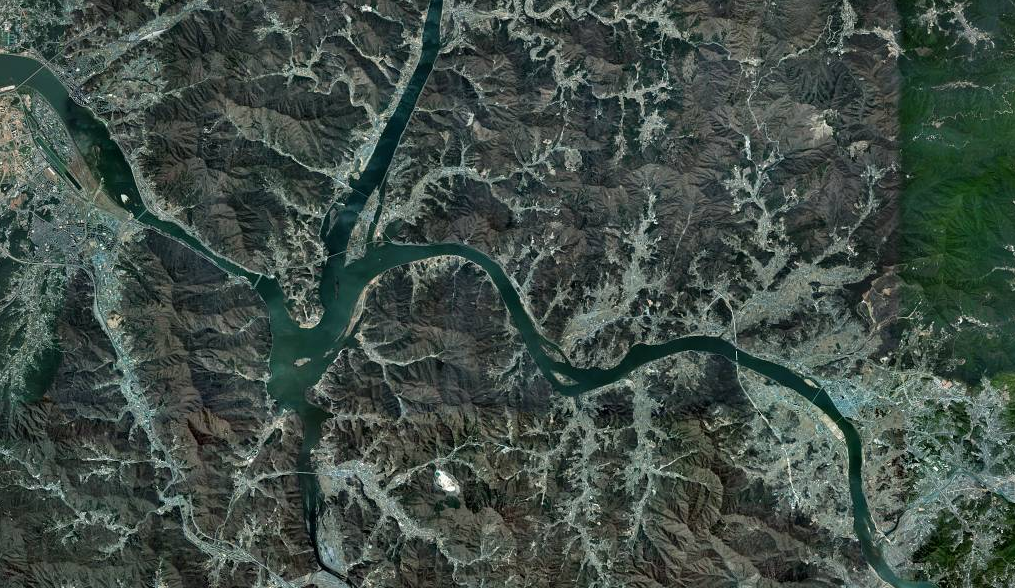
\includegraphics[width=0.6\textwidth]{img/팔당호지도.png}
    \caption{팔당댐 일대의 위성사진. 산이 많다.\protect\footnotemark}
    \label{fig:my_label8}
\end{figure}
\footnotetext{\href{http://kko.to/uvQkz9mYj}{카카오맵 갈무리}}


광주산맥의 험한 산세를 뚤고 지나가다 보면 두물머리라는 곳을 지나가게 된다. 이 곳은 북한강과 남한강이 만나는 곳이다.
바로소 이곳에 와서야 한강이라는 이름을 걷게 된다.
과거, 두 물길이 만나는 곳 답게 크게 번창했으며, 1973년 팔당뎀이 설치되고 일대가 그린벨트로 지정되자,
나루의 기능을 잃었다.
이곳은 TV, 드라마 등으로 널리 알려졌으며,
수변공원이 조성되어 있어 사진 촬영 장소로 인기가 많다.
\footnote{\href{https://terms.naver.com/entry.naver?docId=1997444&cid=42856&categoryId=42856}{양평 두물머리 $|$ 대한민국 구석구석, 2021.01.08, 헌국관광공사}}

\subsection{정보}
\begin{itemize}
    \item 요금: 무료
    \item 연중무휴
    \item 위치: 경기 양평군 양서면 양수리
\end{itemize}


\subsection{팔당댐}
쭉 자전거길을 따라 북한강을 넘고 능내역 터를 지나면, 팔당댐이 그 웅장한 모습을 드러낸다. 
팔당댐 관리교가 댐 양쪽을 이어주지만, 이 다리는 자동차만 통행할 수 있다.


 
\footnotetext{\href{https://memory.library.kr/items/show/20707}{방류중인 팔당댐 $|$ 한국정책방송원, 2005.07.09}}
\begin{figure}
   \centering
   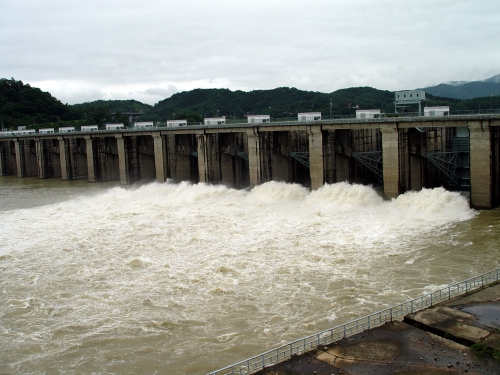
\includegraphics[width=.4\textwidth]{img/팔당댐.jpg}
   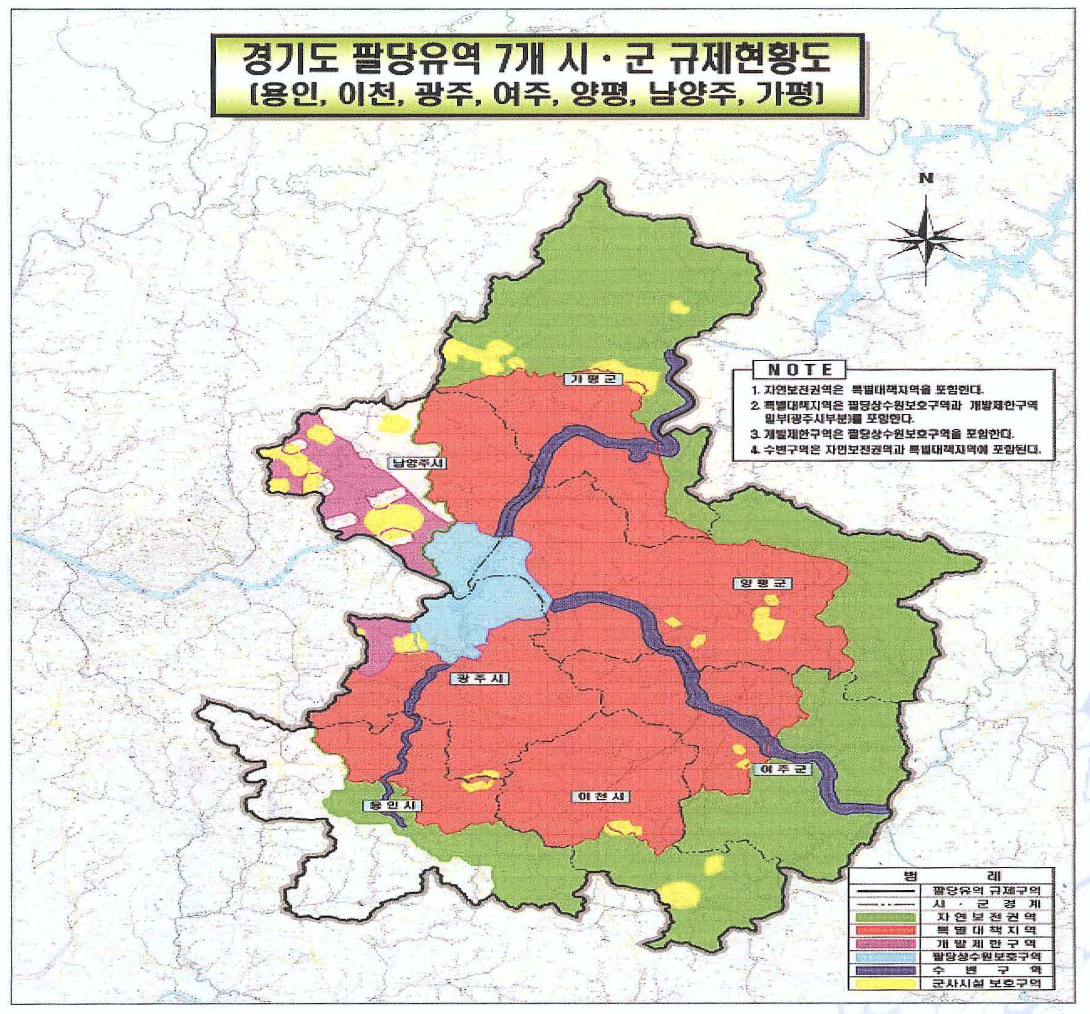
\includegraphics[width=.4\textwidth]{img/규제현황도.PNG}
    
   \caption{(좌)집중호우로 인해 수문을 개방한 팔당댐\protect\footnotemark $\quad$ (우)팔당댐 주변 규제 현황도\protect\footnotemark}
   \label{fig:my_labe9}
\end{figure}
\footnotetext{\ref{paldang}}


팔당댐은 경기도 하남시 천현동과 남양주시 조안면을 잇는
높이 $29m$, 길이 $510m$, 저수량 2억 4400$t$, 유역면적 $23,800km^2$의 콘크리트 중력식 다목적댐이다.
1966년에 착공하여 1973년 12월에 준공되었다.
담수는 1973년 11워 15일 완료되었다.
$17,396,593 m^2$, $11,349$필지가 수몰되었으며, $2,587$만원의 보상액이 지급되었다.
이 댐에는 연간 8만㎾의 수력발전 설비가 설치되어 있다.
\footnote{\href{https://terms.naver.com/entry.naver?docId=531161&cid=46631&categoryId=46631}{팔당댐 $|$ 한국민족문화대백과, 한국학중앙연구원}}


또한 이 팔당호의 팔당취수장에서 얻은 물은 수도권 전역으로 공급된다.
그래서 이 일대와 상류 지역은 "개발 제한구역", "상수원 보호구역", "자원보전권역" 
등으로 지정되어 있으며,
이 일대의 토지주들은 재산원 행사에 제약을 받고 있다.
오수, 폐수, 축산폐수 배출시설은 이 일대에 들어올 수 없다.
이천 하이닉스 반도체 공장이, 이 규제로 인해 증설에 어려움을 겪고 있다.
이는 현재 경기 동부 지역의 발전을 저해하는 요소로 여겨지고 있다.
\footnote{\label{paldang}\href{https://memory.library.kr/items/show/37492}{피해 사례와 개선 방안 ; 팔당상수원 규제 30년 6p, 17p, 29p $|$ 경기도, 2008.07}}
그리고 여름철 집중호우때, 한강의 수위를 조절하는 최종적인 역할도 맏는다.

\subsection{정보}
\begin{itemize}
    \item 요금: 무료
    \item 연중무휴
    \item 위치: 경기 남양주시 조안면 - 경기 하남시 배알미동
\end{itemize}
\chapter{2일차, 한강 하류 (서울 , 인천)}
\section{한강공원}
한강 공원은 서울특별시에서 한강종합개발계획의 일환으로 과거와 같이 깨끗한 강으로
되살리자는 목표로 만들어진 공원이다. 1982년부터 1986년까지 공사되어, 한강의 서울
지역 41.5km 구간인 하일동과 개화동을 잇는 지역이 평균 수심 2.5m, 강너비 1km 의
강으로 변했다. 강변에는 시민 휴식공원, 축구장, 배구장, 농구장, 수영장, 게이트볼장, 
체육시설, 자연학습장, 수상스키장, 수상택시승강장, 요트장, 보트장, 낚시터, 주차장 등 다양한
공간을 갖추어 시민들의 휴양지로 이용할 수 있게 되어 있다.

\begin{figure}[ht]
    \centering
    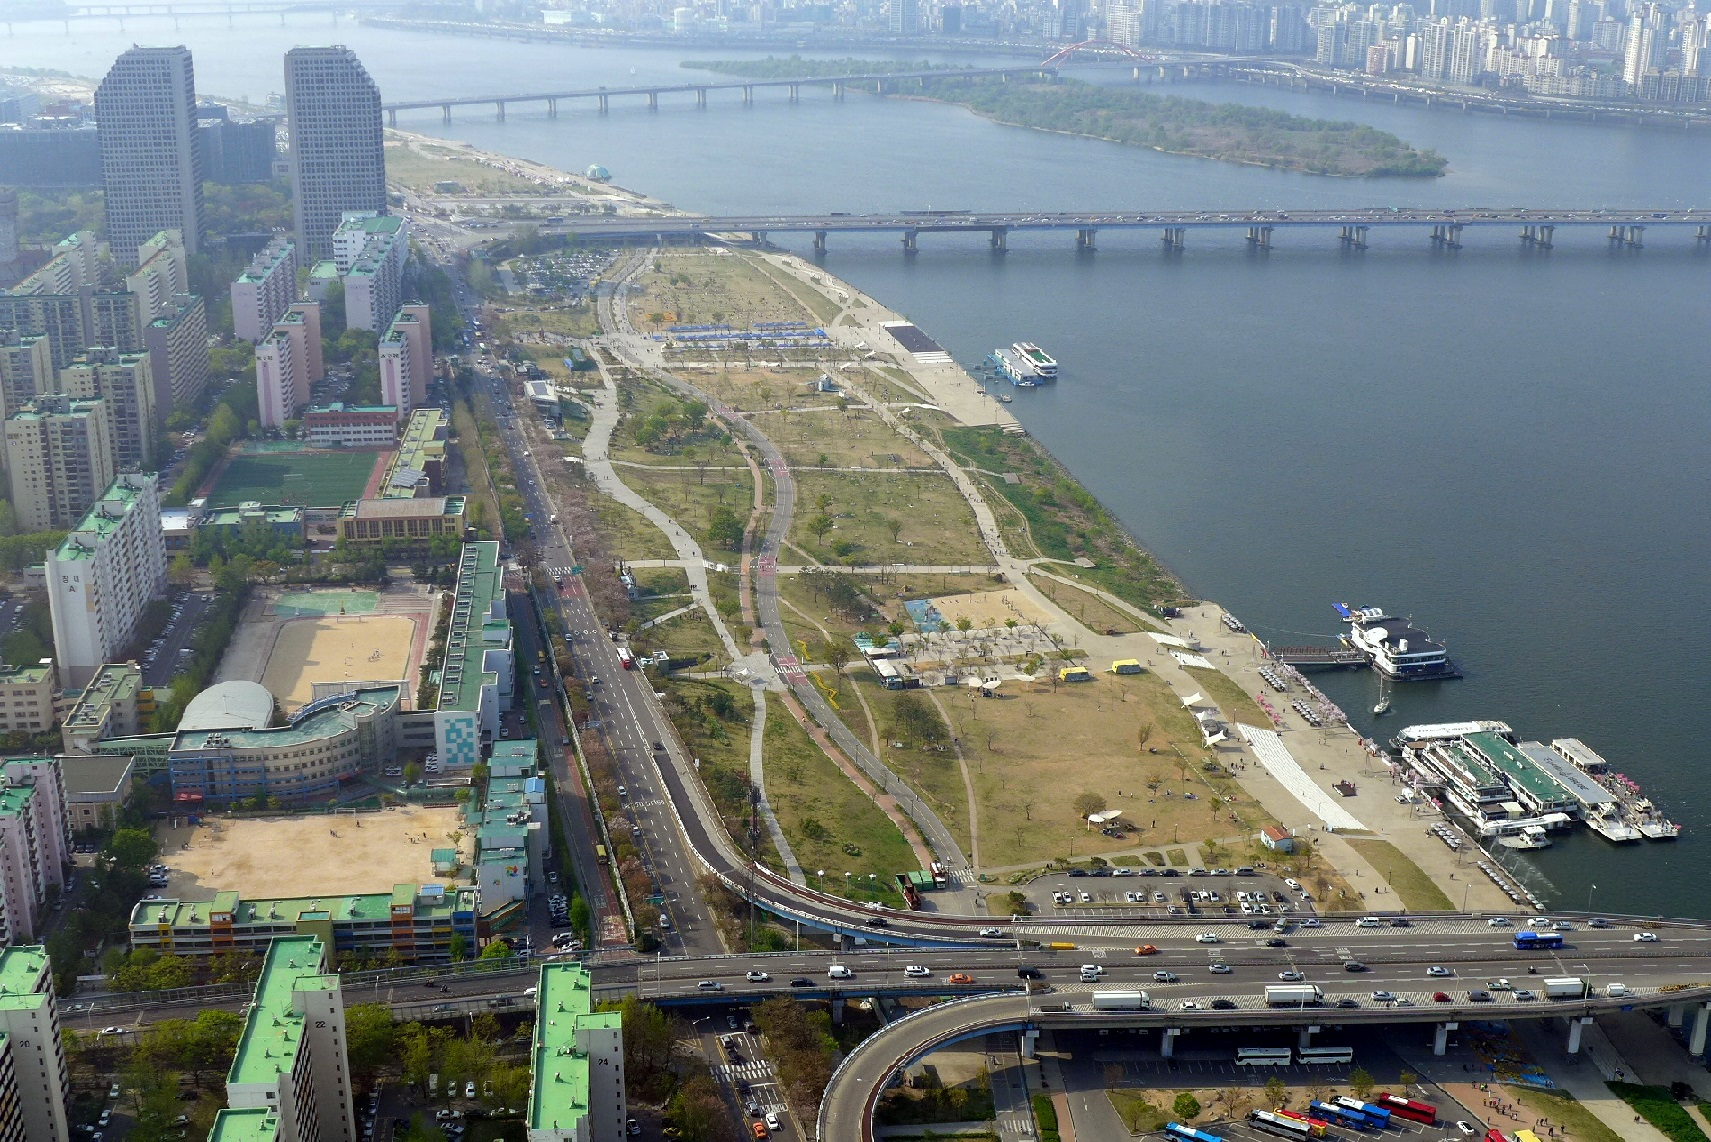
\includegraphics[width=.45\textwidth]{e_img/ww_-000_low.jpg}
    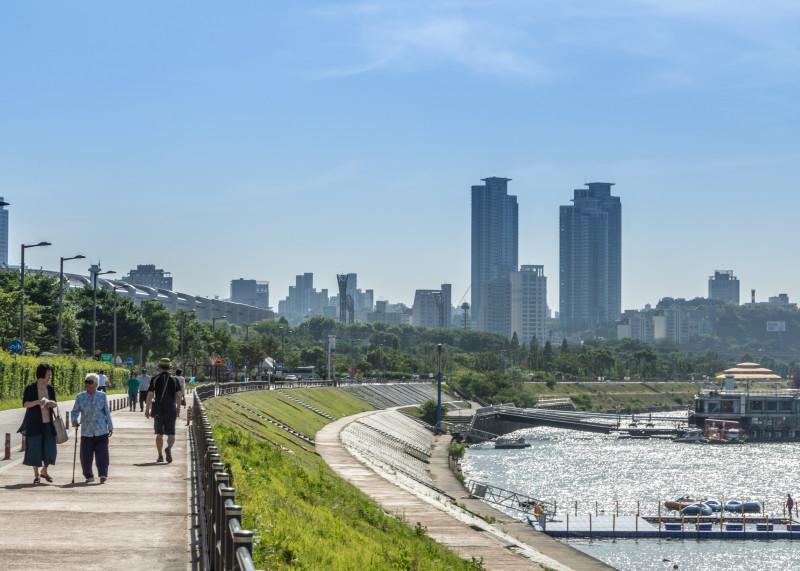
\includegraphics[width=.45\textwidth]{e_img/ww_-001.jpg}
    \caption{(좌) 드론에서 본 서울한강공원 $\quad$ (우)한강공원의 자전거길}
    \label{fig:haryu1}
\end{figure}

한강공원은 걸쳐진 지역에 따라 광나루 한강 공원, 잠실 한강 공원, 뚝섬 한강 공원,
잠원 한강 공원, 반포 한강 공원, 이촌 한강 공원, 여의도 한강 공원, 양화 한강 공원, 
망원한강 공원, 난지 한강 공원, 강서 한강 공원으로 나뉜다. 서울함 공원은 망원 한강 공원에
위치하여 있으며, 잠원 한강 공원 부근에 있는 스타벅스 서울웨이브아트센터점은 물 위에 
떠서 한강뷰를 관람할 수 있는 한강의 대표적인 명소다.

\begin{figure}[ht]
    \centering
    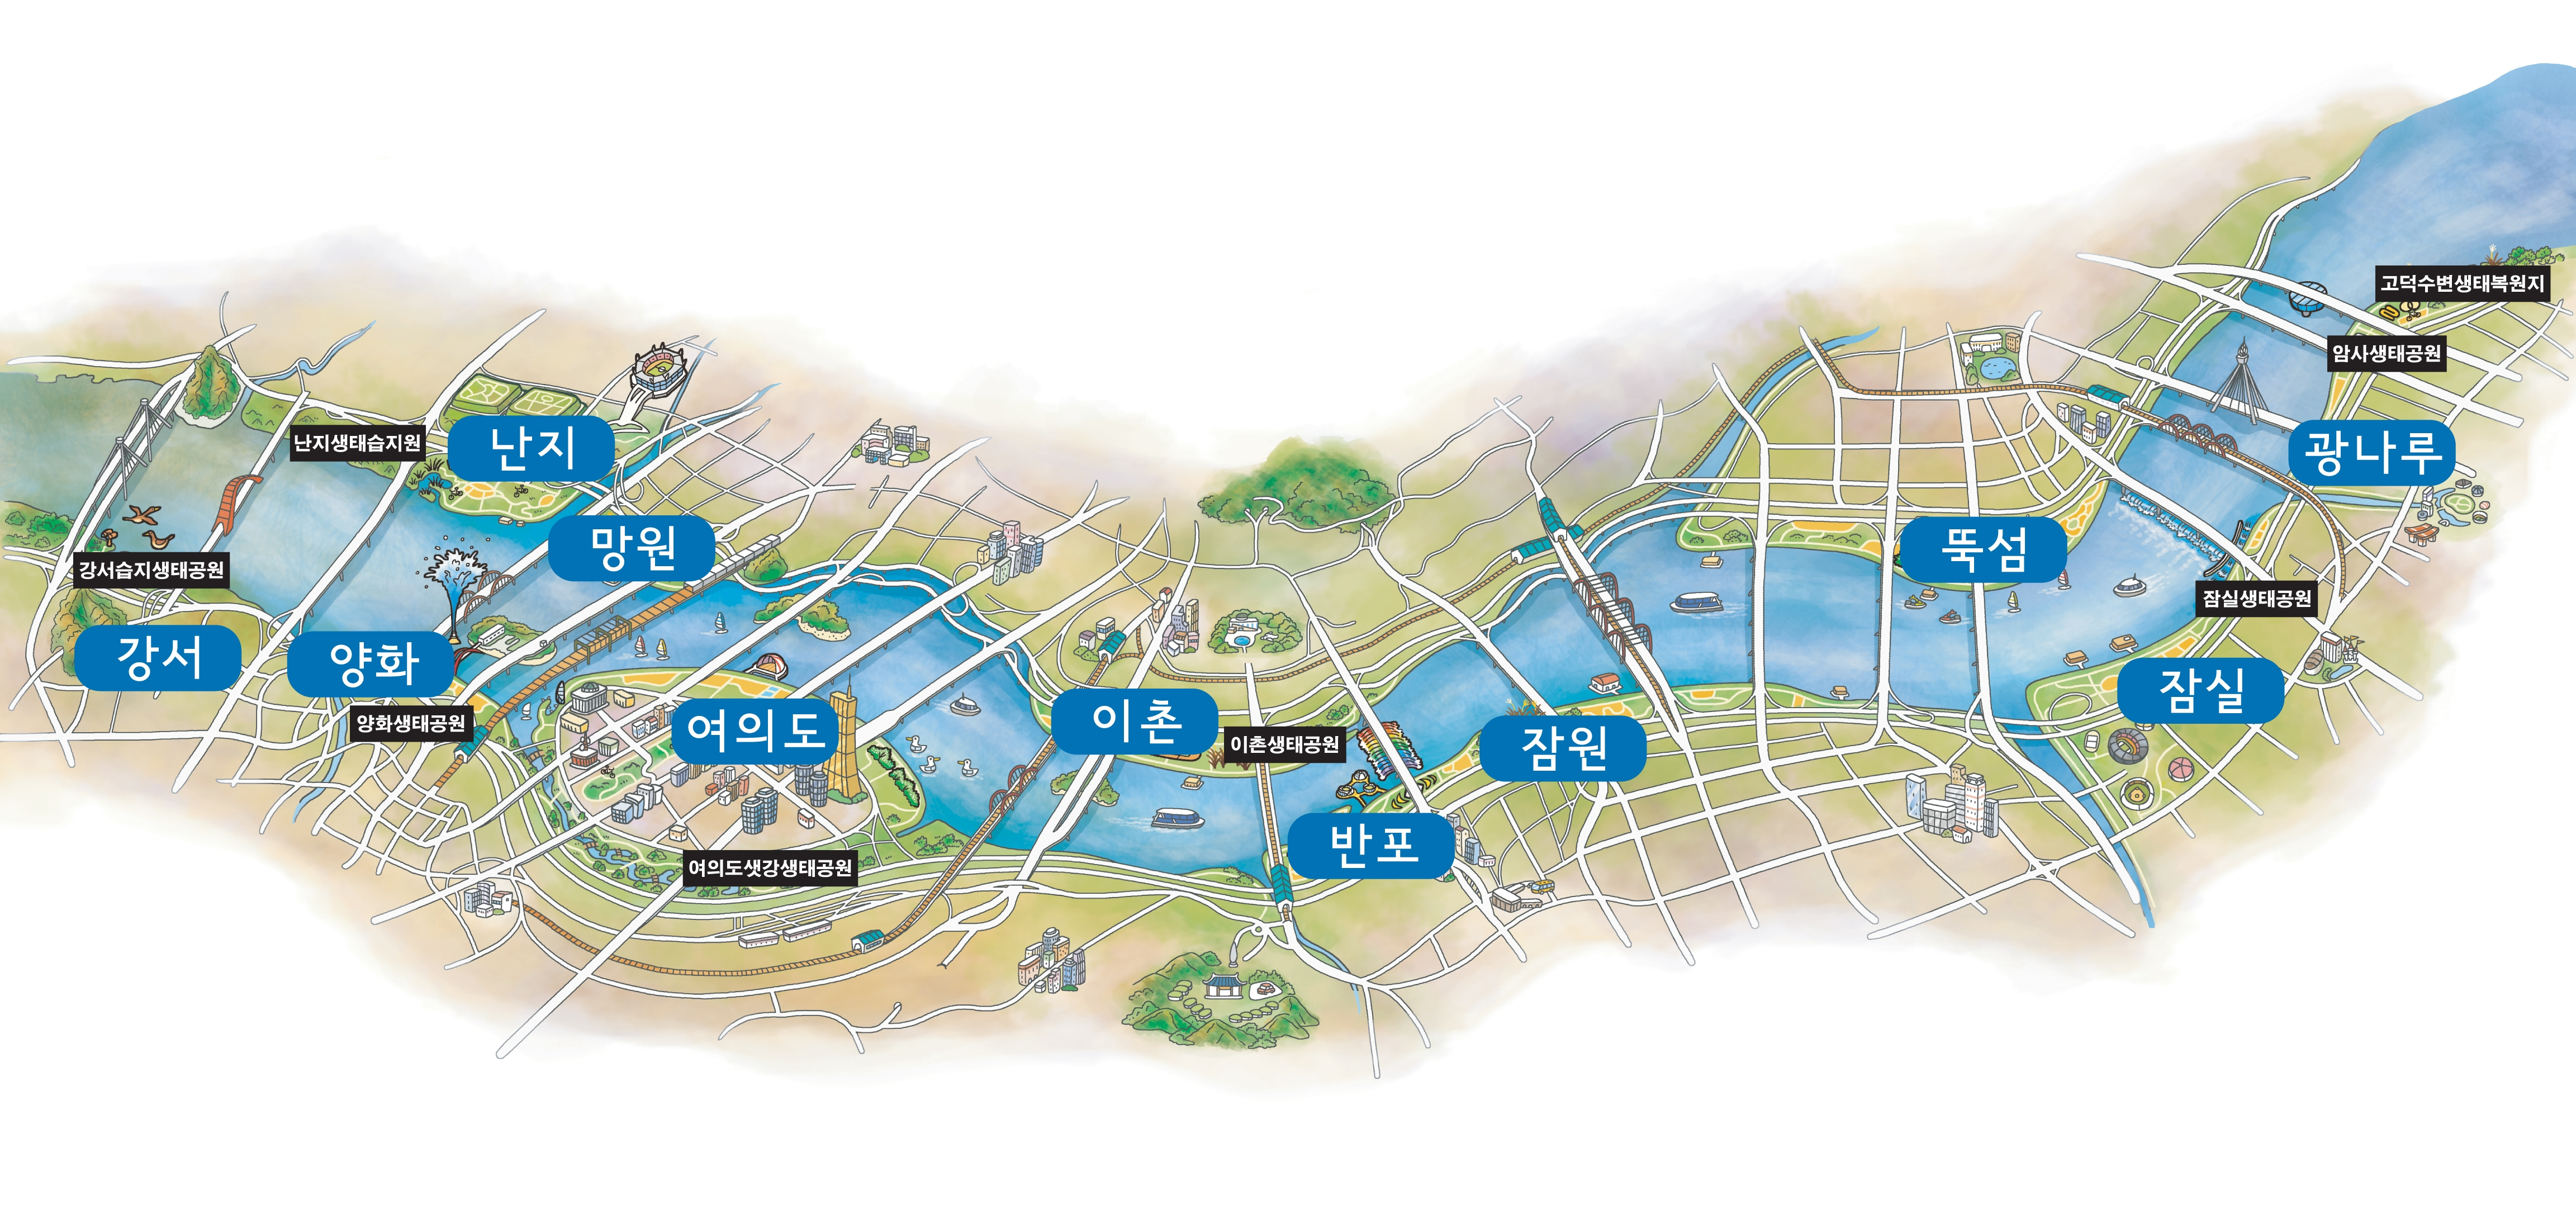
\includegraphics[width=.6\textwidth]{e_img/hanriver.jpg}
    \caption{서울의 한강공원 목록\protect\footnotemark}
    \label{fig:haryu2}
\end{figure}
\footnotetext{\href{https://hangang.seoul.go.kr/archives/9995}{서울시 한강사업본부 $>$ 한강 즐기기 $>$ 한강공원지도, 2019}}

과거의 한강 공원 지역은 강의 수위가 높을 때 잠기는 부지라고 하여 고수부지라고 
불렀으며, 80년대와 90년대에는 고수부지라는 단어가 곧 한강공원을 일컫는 단어이기도 
하였다. 그러나 고수위라는 표현은 일상적으로 잘 쓰이지 않는 용어이고, 부지가 일본식 한자
라는 비판을 받아 한강 둔치라고 고쳐 부르게 되었다. 둔치란 물가에 있는 언덕이라는 
뜻의 단어라서 강가뿐 아니라 바닷가, 호숫가에도 쓸 수 있기 때문에, 보다 정확한 표현으로
한강턱이라고 불러야 한다는 의견도 있다.



법적으로 공원녹지에 해당하며, 서울특별시 한강공원 보전 및 이용에 관한 기본조례,
서울특별시 한강공원 보전 및 이용에 관한 기본조례 시행규칙, 구리시 한강시민공원 이용시설의
설치 및 운영에 관한 조례, 구리시 한강시민공원 이용시설의 설치 및 운영에 관한
조례 시행규칙 등의 보호를 받고 있다.
\footnote{\href{https://ko.wikipedia.org/wiki/한강공원}{한강공원 $|$ 한국어 위키피디아. 2021.06.03 확인}}


\subsection{편의시설 정보}
각종 체육시설과 휴게시설이 있으며, 한강 유람선을 탈수 있는 선착장 등이 있다. 자전거
길이 잘 되어 있기 때문에 서울에서 자전거를 즐겨타는 사람들이 자전거 산책 목적으로
즐겨찾는 공간이기도 하다. 중간에 편의점들이 있는데, 봉지라면을 즉석으로 끓여주는
기기가 갖추어져 있어 이렇게 먹는 라면이 한강 라면으로 유명해지기도 했다. 봉지 라면을
뜯은 뒤, 은박지 그릇 위에 면과 스프를 넣고 물을 넣고 끓여서 먹는 방식이다. 맥주 집도 
들어서서 자전거를 옆에 두고 치맥을 즐길 수 있다.

\begin{figure}[ht]
    \centering
    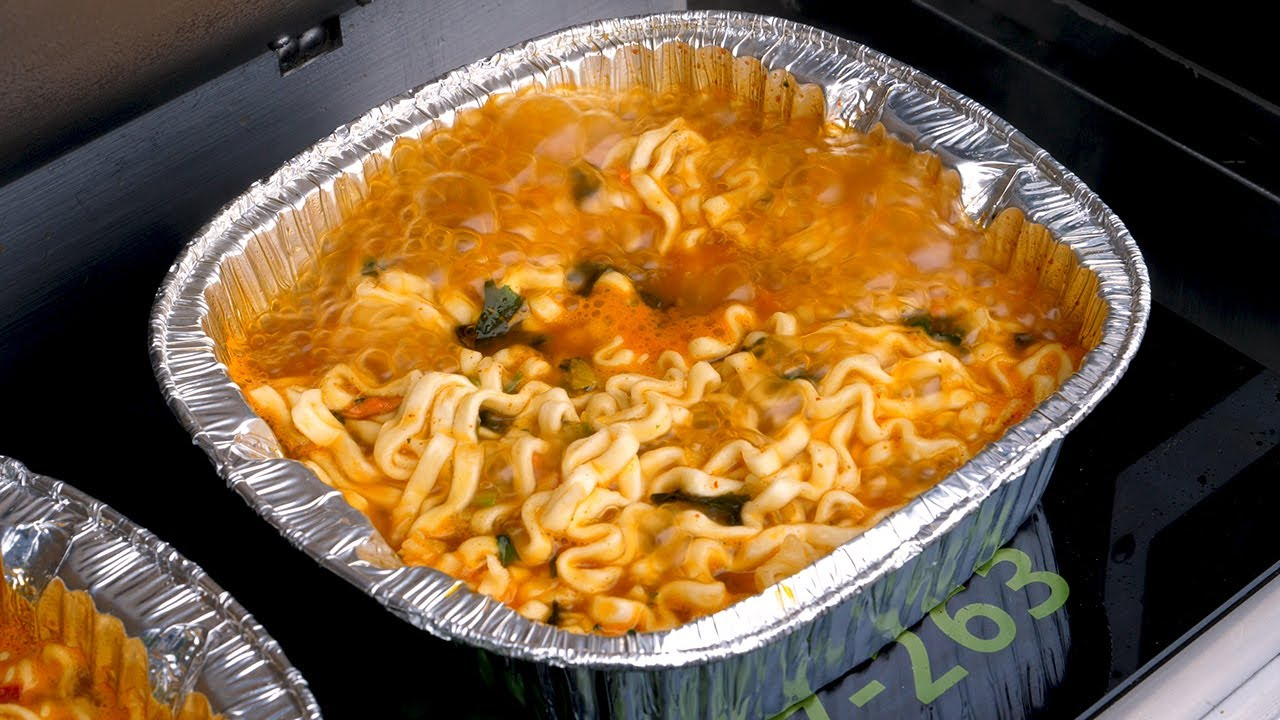
\includegraphics[width=.6\textwidth]{e_img/ww_-003.jpg}
    \caption{한강공원에서 판매하는 라면}
    \label{fig:haryu4}
\end{figure}

주말 오후에 한강 공원을 방문하면 산책로를 따라걸으며 데이트하는 커플들과 자전거를
타고 운동하는 사람들을 많이 볼 수 있다. 단 이 곳 자전거로는 시속 25km 이상의
전기 자전거나 전동킥보드는 허용하지 않으니 알아두어야 한다.

한강 둔치에 위치한 공원은 한강 공원 말고도 많지만 서울특별시에서 한강종합개발계획으로
조성한 공원만 한강 공원이라고 부른다. 때문에 경기도 한강 둔치에 위치한 구리
한강시민공원이나 남양주 한강시민공원 등은 한강공원에 속하지 않는다.


\section{한성백제 역사 유적}
송파구에 위치한 풍납토성과 몽촌토성은 서울에서도 보기 드문 훌륭한 산책 코스 중
하나인데, 이 길은 한국의 고대사에서 아주 중요한 문화유적지이고 백제의 중심지기도 했다.
고즈넉한 산책로를 걸으며 2천 년 전 백제가 꿈꾸던 서울을 알아보자.
이 탐방로의 대부분이자 가장 핵심구간이라고 할 수 있는 곳은 천호역에서 나오면 바로
만나는 풍납토성과 올림픽공원으로도 잘 알려진 몽촌토성이다. 두 개의 토성은 한국의
고대국가로 번성했던 백제의 왕성인 것이다.


백제는 지금부터 약 2000년 전 서울의 한강을 중심으로 건국해 660년에 멸망하기까지
약 700년의 역사를 가진 나라이다. 백제는 고구려, 신라와 함께 한반도에 삼국시대를
이루었으며, 가장 화려한 문화를 꽃피운 나라로 볼 수 있다. 한때 백제가 차지한 한강 유역은
일찍부터 철기문화와 농경문화가 발전해서, 백제는 다른 나라에 비해 상대적으로 풍요롭게
살 수 있었고, 이를 바탕으로 화려한 문화 예술이 발전하였다. 또 서해바다로 이어진
한강을 끼고 있던 백제는 조선기술을 발전시켜 동북아시아 해상교역의 중심국가로 부상할
수 있었다.


백제가 고구려에 패해 수도를 부여로 옮기기 전까지, 서울 송파 지역은 백제의 수도
로서 핵심 요지의 역할을 수행했다. 백제는 4세기 경 근초고왕 때에 이르러 가장 넓은 영토와 
외교적 역량을 가진 강력한 나라가 되었는데, 그 영향력이 한반도의 북쪽으로는 평양에
서 남쪽으로는 가야에 이르렀고, 일본의 규슈 지역, 중국의 요서, 산둥 지역까지 그 영향력
을 뻗쳤다고 알려져 있다 .풍납토성은 바로 이 한성백제의 초기 왕성으로 알려져 있으며,
몽촌토성은 이후에 군사 방어적 목적으로 추가로 건축된 왕성으로 밝혀져 있다. 사실 이러한
역사적 사실이 제대로 밝혀지고 알려진 것은 얼마 되지 않았다. 1997년 풍납토성에서
대규모의 유물이 출토되기 전까지 풍납토성과 몽촌토성은 백제의 성이기는 하지만 그리 
중요한 성일 것이라고 아무도 생각하지 않았다. 그러나 풍납토성에서 대규모의 백제의 
왕궁유물이 출토되면서 많은 역사학자들이 궁금해 했던 백제 초기의 왕성이 1600여 년 만에
드러난 것이다. 그래서 이 탐방로의 구간은 최근까지도 활발한 발굴과 연구조사가 진행 
중이기도 하다.

\subsection{풍납토성}


풍납토성은 그 규모와 건축 기술에서 고대 이집트의 피라미드 건축 기술을 뛰어 넘는
다. 풍납토성은 판축기법과 부엽공법을 사용해 만들었는데, 이것은 일정한 간격으로 만든
나무틀에 체로 거른 고은 흙과 나뭇잎, 그리고 뻘흙을 사용해 시멘트보다 단단한 토성을 
만들어낸 방식이다. 발굴 과정에서 드러난 풍납토성의 규모도 입을 다물지 못할 수준이다. 
풍납토성은 최대 폭이 40m, 높이 15m, 배 모양의 성곽이 3.5km 길이로 이어져 있다. 이 정도
공사를 하기 위해 10톤 트럭 15만 대(150만 톤) 분량의 흙이 필요하고, 연간 200만 
명이 동원되었을 것으로 추정된다. 백제가 초기부터 강력한 왕권 국가가 아니었다면 해낼 수
없는 대규모 국책 사업이었던 것이다.
\footnote{\href{https://ko.wikipedia.org/wiki/서울_풍납동_토성}{서울 풍납동 토성 $|$ 한국어 위키피디아. 2021.06.03 확인}}

\begin{figure}[ht]
    \centering
    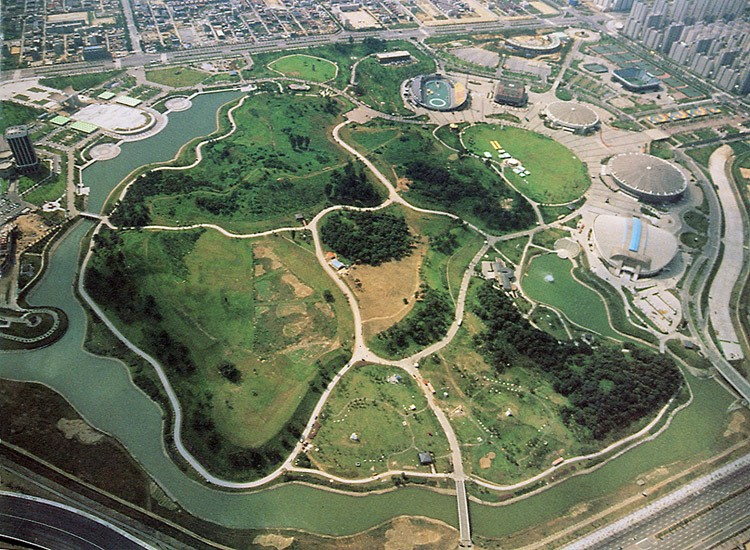
\includegraphics[width=.45\textwidth]{e_img/ww_-004.jpg}
    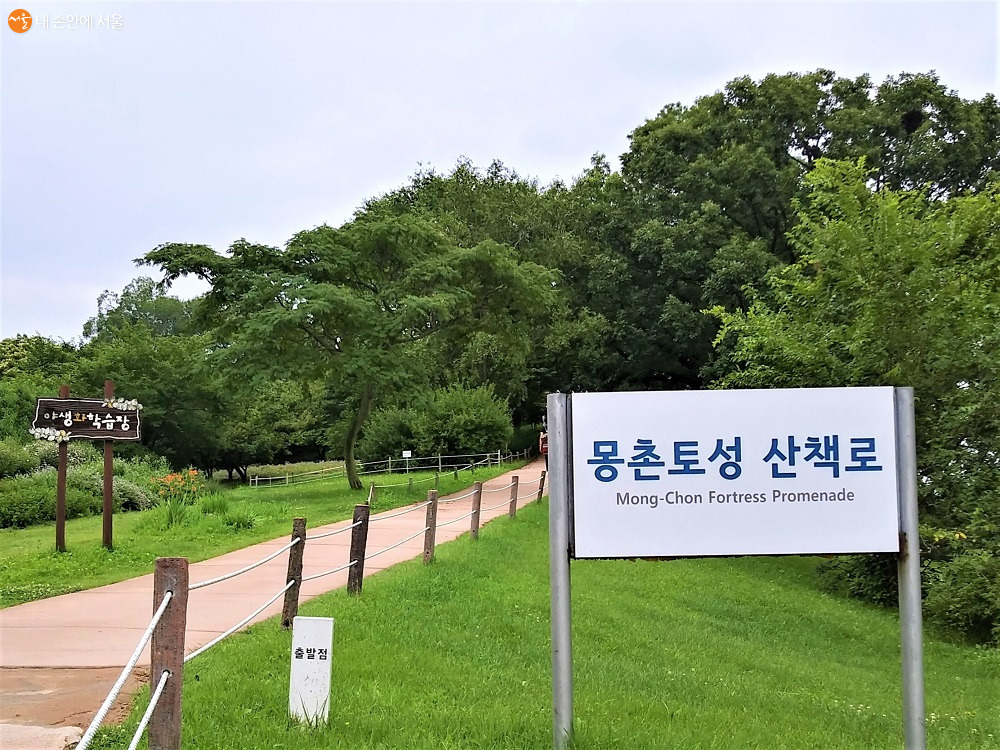
\includegraphics[width=.45\textwidth]{e_img/ww_-005.jpg}
    \caption{풍납토성(좌)와 몽촌토성(우)}
    \label{fig:haryu6}
\end{figure}

\subsection{몽촌토성}
몽촌토성은 근초고왕 시기인 4세기 전후에 축조된 백제의 왕성으로, 남한산성의 
산줄기와 한강의 자연지형을 그대로 이용해 건축되었다. 몽촌토성의 호수 역시 자연지형을
이용해 만든 해자의 흔적이다. 비록 지금은 지형이 많이 바뀌었지만, 옛 지도를 보면 
몽촌토성의 호수는 현재의 석촌 호수까지 이어져 한강의 지류를 이루고 있었다. 몽촌토성을 
만든 이유에 대해서는, 위례성의 인구가 증가하자 위례성 밖에 살고 있는 백성들을 위해 
축조했다는 의견과 함께, 초기 왕성인 풍납토성이 적의 공격에 취약해 방어성으로서 몽촌토성
을 새로 건축했다는 의견도 힘을 얻고 있다. 어찌되었든 풍납토성과 함께 몽촌토성은 
백제가 강력한 고대 국가의 기틀을 다질 수 있게 해준 왕성으로 평가받고 있다.
\footnote {\href{https://ko.wikipedia.org/wiki/서울_몽촌토성}{서울 몽촌토성 $|$ 한국어 위키피디아, 2021.06.03 확인}}



\section{선유도 공원}
방탄소년단 멤버 RM 의 `seoul'이라는 곡을 들어보면 가사에 선유도가 등장한다. 서울
사람에게 선유도 공원은 꽤 중요한 장소임이 틀림없다. 양화대교와 맞닿아 있으며, 
행정구역 상으로 영등포구 당산동과 양화동에 속해 있다.

한강 중심부에 자리한 작은 봉우리섬 선유도는 예로부터 빼어난 풍광을 지닌 곳으로
예술가와 묵객시인들의 사랑을 받은 곳이었다. 그러나 일제강점기를 거치며 선유봉의 옛
모습은 사라졌고, 1978년부터 2000년까지 서울 서남부 지역에 수돗물을 공급하는 
정수장으로 사용되었다. 이후 2002년 4월 다양한 볼거리와 즐거움을 선사하는 
친환경생태공원으로 재생되었다.


\begin{figure}[ht]
    \centering
    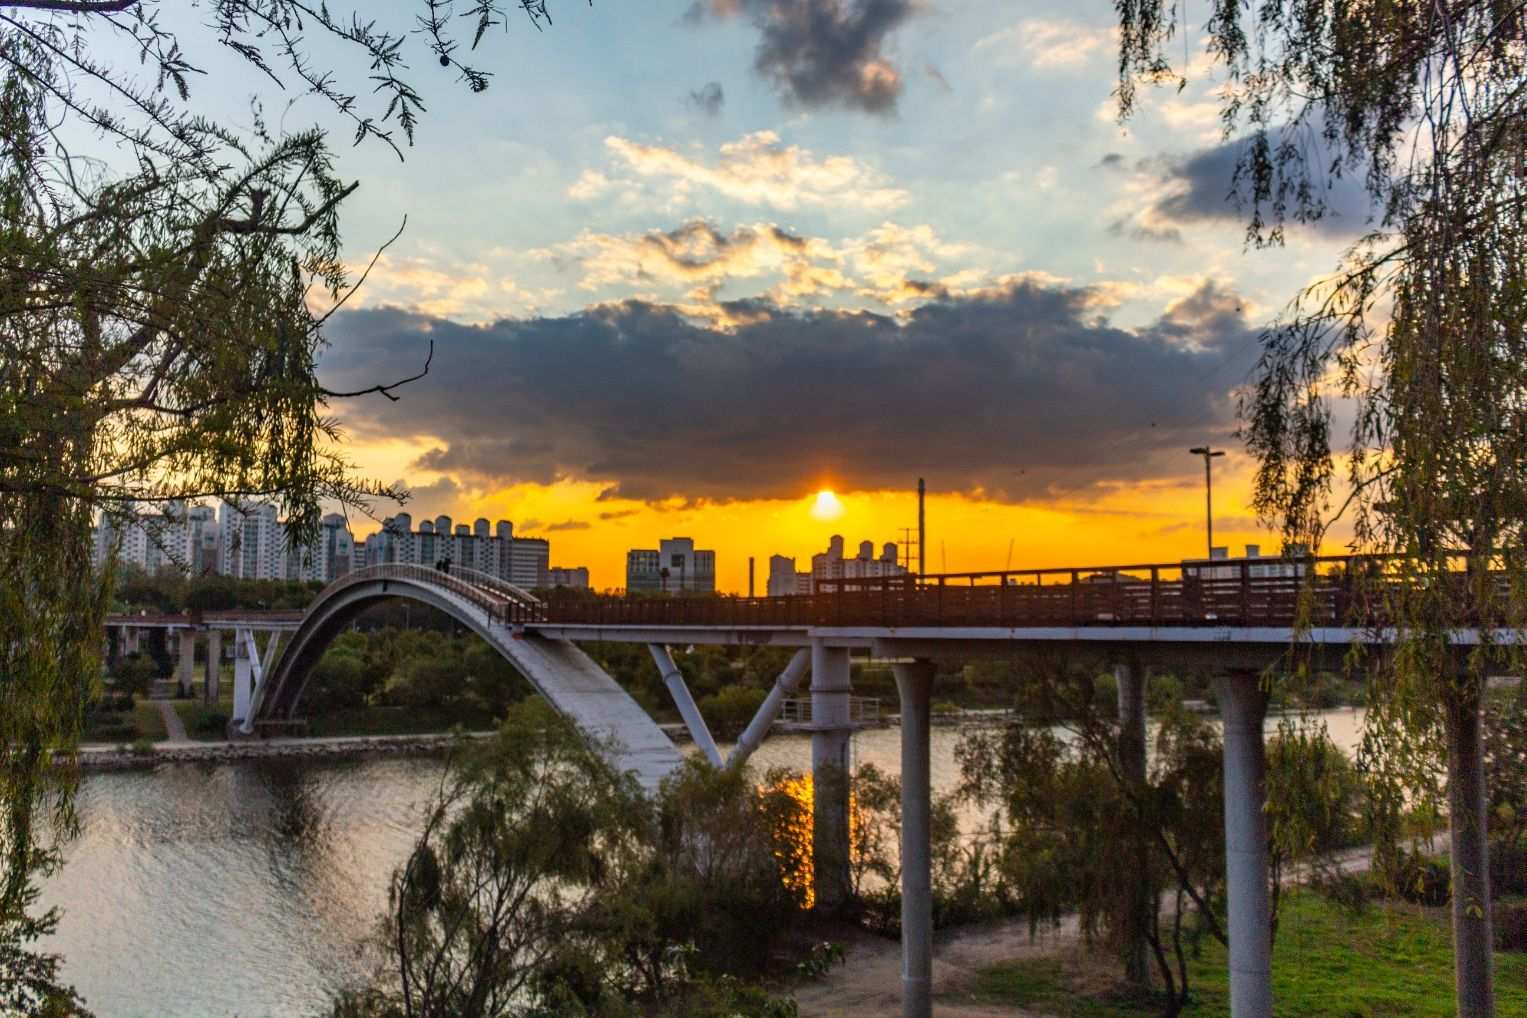
\includegraphics[width=.55\textwidth]{e_img/ww_-006.jpg}
    \caption{선유도 공원의 일몰}
    \label{fig:haryu7}
\end{figure}

카페와 식당이 안에 있다. CU 편의점 선유도점이 열었다가 문을 닫았고, 지금은 
나루라는 카페테리아가 영업 중이다. 커피 맛에 민감한 사람이라면 추천하지 않는다. 한강 
건너편에는 한강시민공원 양화지구가 있다. 무지개다리라 불리는 선유교를 통해 직접 건널 수
있으며, 야간이 되면 무지개빛 형광을 띠는 볼거리를 선사한다. 비탈길을 갖추어 놓았지만
그것은 노약자와 정비차량을 위해 마련된 것으로, 자전거로는 통행할 수 없다.


이 외 한강전시관, 수질정화원, 환경물놀이터, 녹색 기둥이 있는 정원, 수생식물원,
시간의 정원,원형소극장 등의 공간을 볼 수 있다. 선유도는 느즈막한 노을 시간대와 밤 
시간대의 야경이 특히 아름답다.
\footnote{\href{https://ko.wikipedia.org/wiki/선유도공원}{선유도공원 $|$ 한국어 위키피디아. 2021.06.03 확인}}


\section{저녁: 서울신라호텔 팔선 중식당}


\begin{figure}[ht]
    \centering
    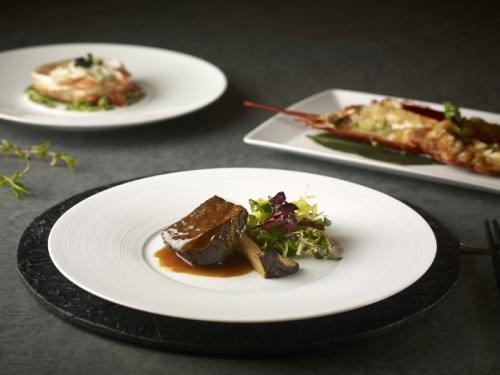
\includegraphics[width=.55\textwidth]{e_img/ww_-007.jpg}
    \caption{팔선 중식당의 코스요리}
    \label{fig:haryu8}
\end{figure}


우리나라 부자들은 대부분 부동산 투자로 부를 축적하였다. 비트코인과 주식이 단기
투자를 통해 엄청난 이득을 낼 수 있는 것 같아도, 주요 도시에 위치한 부동산만큼의 안정
적인 상승세를 보장하지 못한다. 한국의 역사를 관통하고 있는 한강 근처는 서울시에서 
가장 집 값이 높은 지역이며, 교통과 편의 그리고 배산임수가 잘 고려된 대한민국 최고의 
거주지라는 평가를 받는다.

서울을 떠나기 전 고급스럽기로 손에 꼽히는 서울신라호텔 팔선 중식당에서 식사해
보는 것을 추천한다. 중식이지만 한국의 문화가 잘 반영되어 있으며, 영어 등 외국인을 위
한 메뉴판이 준비되어 있다. 세트 메뉴는 인당 20만원 수준으로 가격대가 있는 편이지만,
3만원 이내의 면류나 10만원 이내의 메인 디쉬를 고를 수 있고 이 외에도 선택지가 다양하다.



\section{강화해협}


인천 강화군 강화도는 답사의 일번지, 우리 역사의 전시장 등으로 불리는데, 유적과
유물이 많고, 중요한 역사적 사건이 많이 발생했다. 국내, 국제 무역을 위한 해선들이 
서울로 진입하기 위해 반드시 거쳐야 하는 첫 번째 관문이었다.

\begin{figure}[ht]
    \centering
    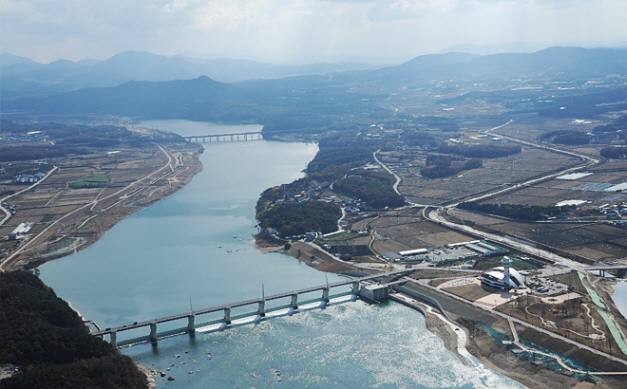
\includegraphics[width=.55\textwidth]{e_img/ww_-008.jpg}
    \caption{강화해협의 모습}
    \label{fig:haryu9}
\end{figure}


한강에 관심 있는 사람이라면 염하라는 말을 들어본 적이 있을 것이다. 염하는 강화
해협을 이르는 말로, 프랑스 병인양요 시기 프랑스의 1차 보복 전 원정 과정 중, 프랑스 신
부와 갑구지 촌로 사이의 잘못된 통역으로 인해 짠 물로 해석되어 지금까지 전해져 내려오
고 있다고 알려져 있다. 서해안의 조수간만의 차가 큰 까닭에 배를 타고 이 곳을 지나기는
쉽지 않으며, 밀물과 썰물 때는 물살이 아주 세차게 흐르는 곳이기도 하다. 해협을 가로질
러 강화대교와 강화초지대교가 해협 위에 건설되어 있다. 과거에는 배를 타고 한강으로 들
어가는 통로였기에 아주 중요한 해상교통로의 역할을 했다. 그 흔적으로 강화해협 주변에
진, 보, 돈대, 포대 등 많은 군사시설들이 산재해 있음을 볼 수 있다.



\chapter{기타}
\section{역할분담}
\subsection{A군}
\begin{itemize}
    \item 주제 제안
    \item 답사 장소 제시
    \item 한강 중류(여주, 이천, 양평, 남양주)에 대해 조사.
    \item LaTeX으로 보고서 합치기
\end{itemize}
\subsection{B군}
\begin{itemize}
    \item 한강 상류(태백, 정선, 단양, 충주)에 대해 조사.
\end{itemize}
\subsection{C군}
\begin{itemize}
    \item 한강 하류(서울, 김포, 강화)에 대해 조사.
\end{itemize}


\section{느낀점}
\subsection{A군}
\begin{itemize}
    \item 요즘은 코로나라 그러지 못하지만, 나는 강가에 가는 것을 어렸을 때부터 좋아했다. 넓고 흐르는게 좋았다. 평소에는 서울이면 서울의 강, 영월이면 영월의 강, 이런식으로 조금씩 보아 왔다. 이 기억의 파편들을 보고서를 통해 합쳐서 강 전체를 조망하게 되어 기뻤다.
    \item LaTeX을 이용해서 보고서를 작성했는데, 거의 사용 방법을 모르기 때문에 여러 문법을 검색을 통해 찾아가면서 재미있게 완성했다. 합친 보고서를 보니 뿌듯하다.
\end{itemize}
\subsection{B군}
\begin{itemize}
    \item 한강 상류(태백, 정선, 단양, 충주)에 대해 조사.
\end{itemize}
\subsection{C군}
\begin{itemize}
    \item 한강 하류(서울, 김포, 강화)에 대해 조사.
\end{itemize}
\end{document}